
%%% Local Variables:
%%% mode: latex
%%% TeX-master: ".."
%%% End:

\section{grid绘图系统}
\subsection{另辟蹊径}
\begin{frame}{\subsecname}{}
  % % \begin{minipage}{\textwidth}
  % %     \begin{ornamentblock}
  % %       { 林尽水源,便得一山,山有小口,仿佛若有光。便舍船,从口入。初极狭,才通人。复行数十步,豁然开朗。土地平旷,屋舍俨然,有良田美池桑竹之属。阡陌交通,鸡犬相闻。其中往来种作,男女衣着,悉如外人。黄发垂髫,并怡然自乐。\\
  % %         \rightline{\textemdash《陶渊明·桃花源记》}}
  % %     \end{ornamentblock}
  % % \end{minipage}
  % % \begin{minipage}{\textwidth}
  % %    \centering 
\includegraphics[width=0.6\columnwidth]{桃花源记.png}
  % % \end{minipage}
  \begin{columns}
    \begin{column}{.5\textwidth}
      \begin{figure}
        \centering 
\includegraphics[width=0.9\columnwidth]{标新立异.jpg}
      \end{figure}
    \end{column}

    \begin{column}{.48\textwidth}
      \begin{ornamentblock}
        \centering
        {支道林在白马寺中;将冯太常共语;因及《逍遥》;支卓然标新埋于二家之表;立异于众贤之外\\
          \rightline{\textemdash《刘义庆·世说新语》}}
      \end{ornamentblock}
      % \curlyframe{工欲善其事,必先利其器\\
      % \rightline{-----《论语·卫灵公》}}
    \end{column}
  \end{columns}
\end{frame}

\begin{frame}[t,fragile]{\subsecname}{}
\begin{itemize}
\item<1-> 前面介绍的graphics程序包是R的标准绘图系统,也称为\emphText{graphics绘图系统},
  除此之外R中还有另一套截然不同的\emphText{grid绘图系统}
\item<1-> 使用grid绘图系统前需要先用\emphText{library(grid)}加载grid程序包,
该程序包由\href{https://www.stat.auckland.ac.nz/~paul/}{\uline{Paul Murrell}}开发维护
%\textsuperscript{\underline{\href{https://www.stat.auckland.ac.nz/~paul/}{主页}}} 
\item<2-> grid绘图系统的\emphText{设计初衷是为了克服graphics系统中元素不能动态修改的弱点}
\end{itemize}

\vspace{-10pt}
\begin{overlayarea}{\textwidth}{\textheight}
\only<1>{
\begin{figure}\centering
  \captionsetup[subfigure]{labelformat=empty} 
  \subfloat[]
  {
\includegraphics[height=0.4\textheight]{paul_murrell.jpg}} \vspace{1pt}
  \subfloat[]
  {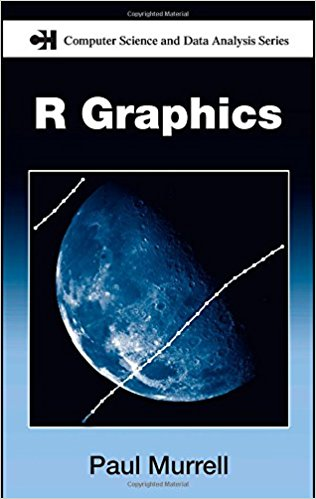
\includegraphics[height=0.4\textheight]{R_graphics_cover.jpg}} \vspace{-10pt}
  \caption{左图是grid作者Paul Murrell,目前是奥克兰大学统计系副教授;右图是他在2005年写的
书—《R Graphics》,现在已成为R领域的经典入门书籍}  
\end{figure}}

\only<3>{
\begin{block}{\small grid系统和graphics系统的区别} \footnotesize
\begin{itemize} 
\item[\HandRight] grid用\emphText{视口(viewports)}将绘图设备分割为不同的区域,
绘图对象(grob)可以在不同的视口中进行共享,比graphics中的处理方式更加灵活
\item[\HandRight] grid绘图对象可以被修改或者从一个图形中移除,\emphText{而不需要重新绘制所有的图形},
但是在graphics中则必须重绘 
\item[\HandRight] grid绘图系统是一个绘图框架,其原生的grid程序包仅提供低级绘图函数用于绘制统计图形中的元素,
不像graphis程序包还集成了高级绘图函数用于绘制常用的统计图形,
因此\emphText{直接用grid程序包绘制统计图形比较繁琐}
\item[\HandRight] \emphText{两套系统的绘图函数和绘图参数完全不同,不能混用!}
\end{itemize}
\end{block}}

\begin{onlyenv}<2>
\begin{columns}
  \begin{column}[t]{.5\textwidth}
    \begin{rcode}
# 基础统计图形库处理方式
plot(0:1, 0:1)
rect(0, 0, 1, 1, col = "red")
# 为了改变颜色,必须重画整幅图形
plot(0:1, 0:1)
# 虽然可以用新的矩形覆盖旧的,但旧矩形仍然存在
rect(0, 0, 1, 1, col = "blue")
    \end{rcode} 
  \end{column}

  \begin{column}[t]{.5\textwidth}
    \begin{rcode}
# grid绘图系统的处理方式
grid.rect(name = "rect0")
# 修改它的填充颜色为红色
grid.edit("rect0", gp = gpar(fill = "red"))
# 修改为蓝色,不需要重新用grid.rect()画矩形
grid.edit("rect0", gp = gpar(fill = "blue"))
    \end{rcode} 
  \end{column}
\end{columns} 
\end{onlyenv}

\only<4>{
\begin{figure}[t]
\centering
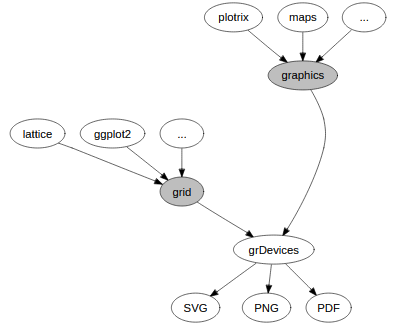
\includegraphics[width=0.45\columnwidth]{grid_system.png}
\caption{\emphText{lattice}和\emphText{ggplot2}是基于grid包开发的绘图程序包,这样就在grid
绘图系统中使用高级绘图函数来简化统计图形的绘制过程}
\end{figure}}
\end{overlayarea}
\end{frame} 

\subsection{lattice程序包}
\begin{frame}[t,fragile]{\subsecname}{}
\begin{itemize}
\item lattice程序包是基于grid包的编写的一套统计图形库,2000年发布了第一个版本,由
\href{https://www.isid.ac.in/~deepayan/}{\uline{Deepayan Sarkar}}等人开发维护,从R 3.0版本开始纳入base包,\emphText{不需要再单独安装}
\item lattice设计理念来自S-PLUS中的Trellis图形,是一种\emphText{多元数据可
视化的方法}:首先将多元数据分类组织,然后将绘图元素都 保存在一个\emphText{trellis对象}中,最后在\emphText{嵌板(panel)}区域绘制该对象,并且在panel上方用
\emphText{条板(strip)}区域来描述分类信息
\end{itemize}

\vspace{-8pt}
\begin{overlayarea}{\textwidth}{\textheight}
\only<1>{
\begin{figure}[ht]
  \centering
  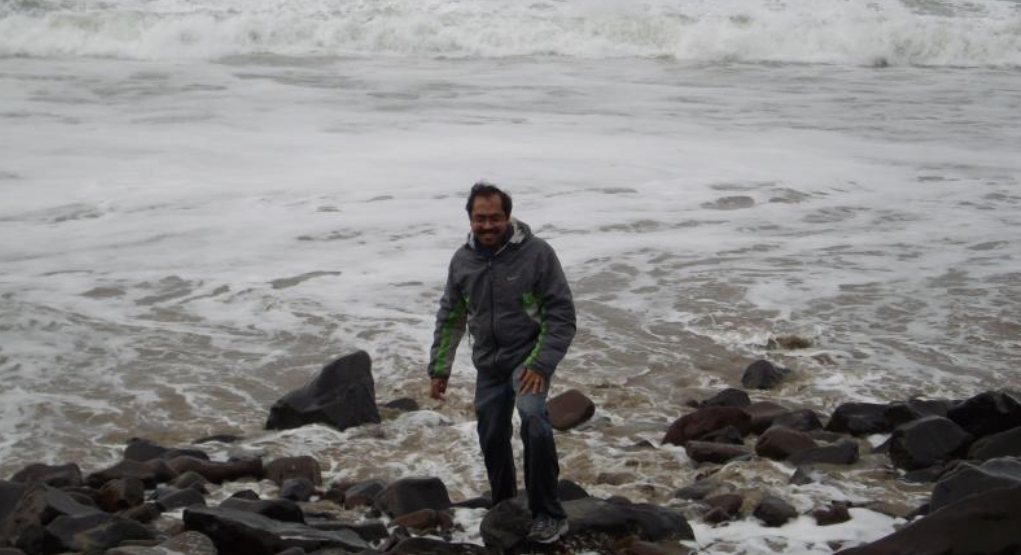
\includegraphics[width=0.7\columnwidth]{deepayan_sarkar.png}
  \caption{lattice程序包作者Deepayan Sarkar,目前是印度统计研究院的研究员}
\end{figure}}

\only<2>{
\begin{figure}[ht]
  \centering
  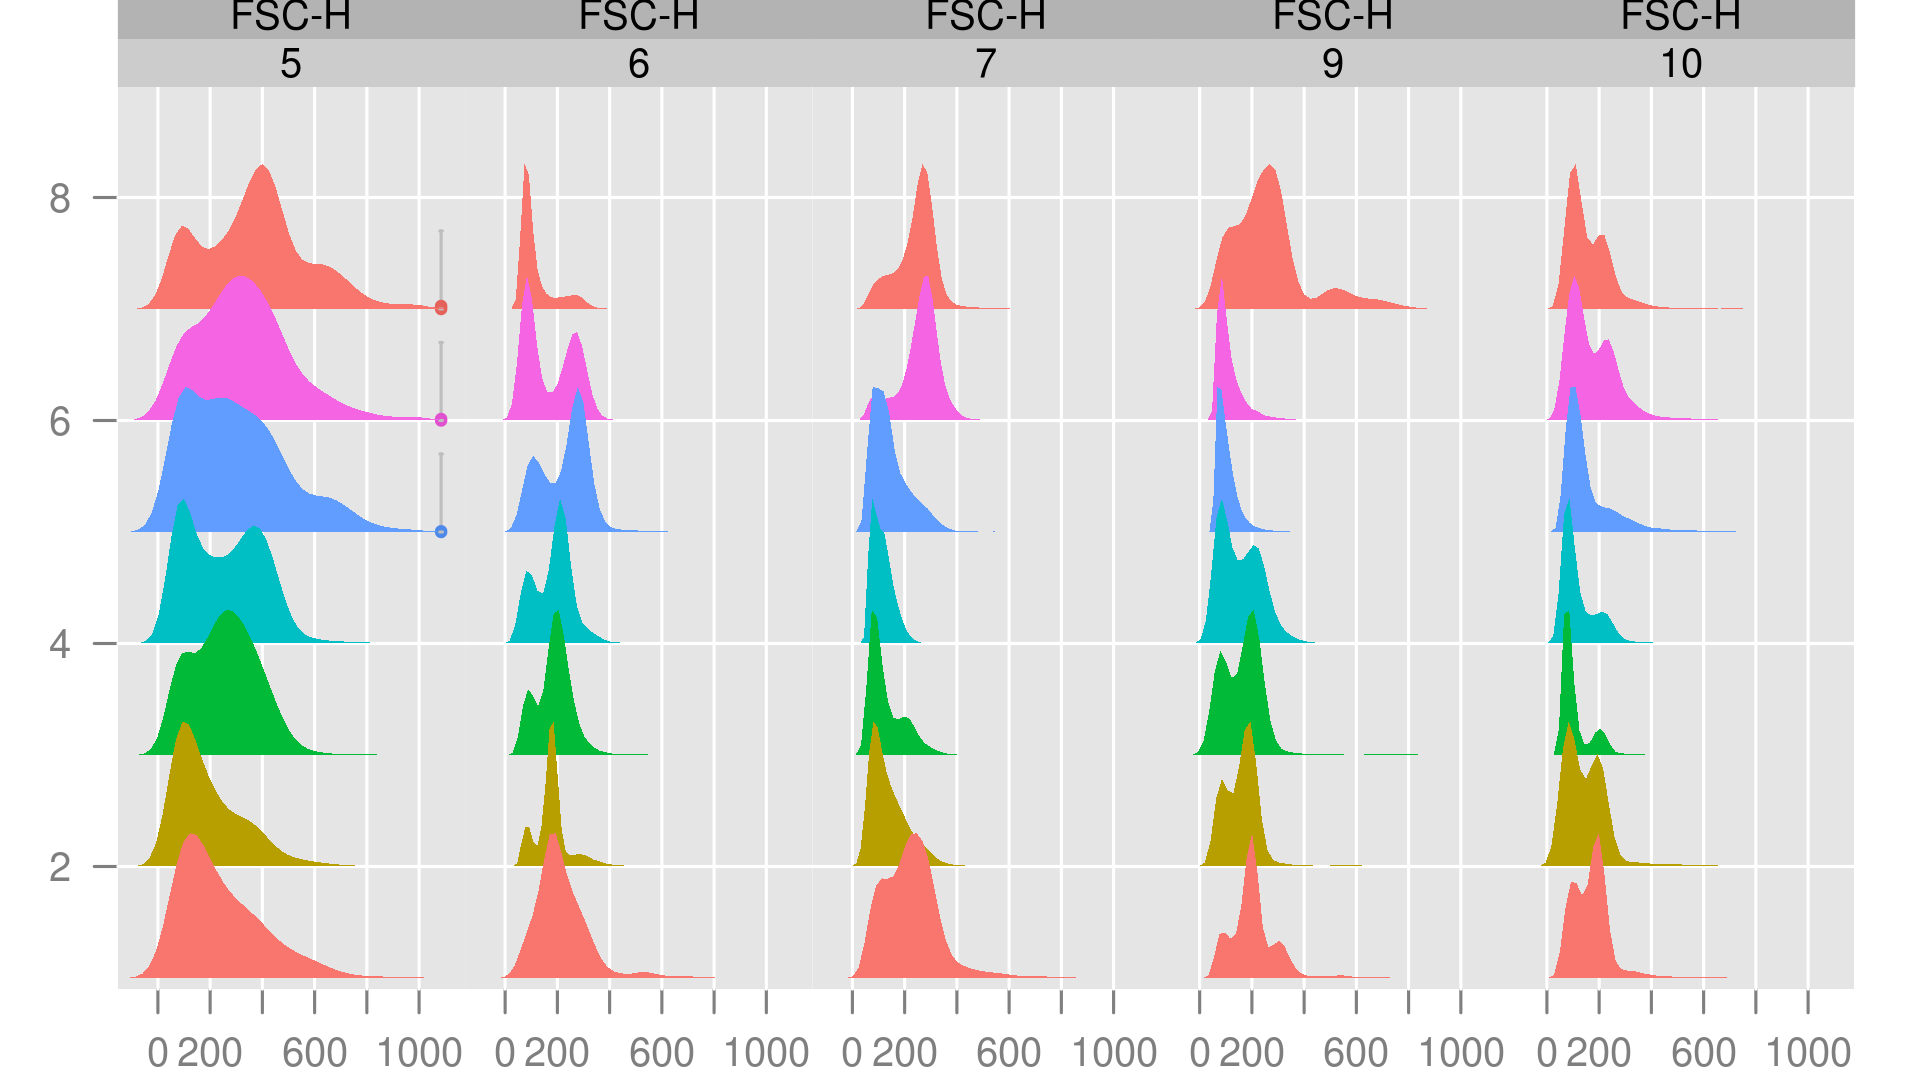
\includegraphics[width=0.7\columnwidth]{lattice-example1.png}
  \caption{不同的GvHD病患者在细胞检测中的FSC-H结果数据}
\end{figure}}

\only<3>{
\begin{figure}[ht]
  \centering
  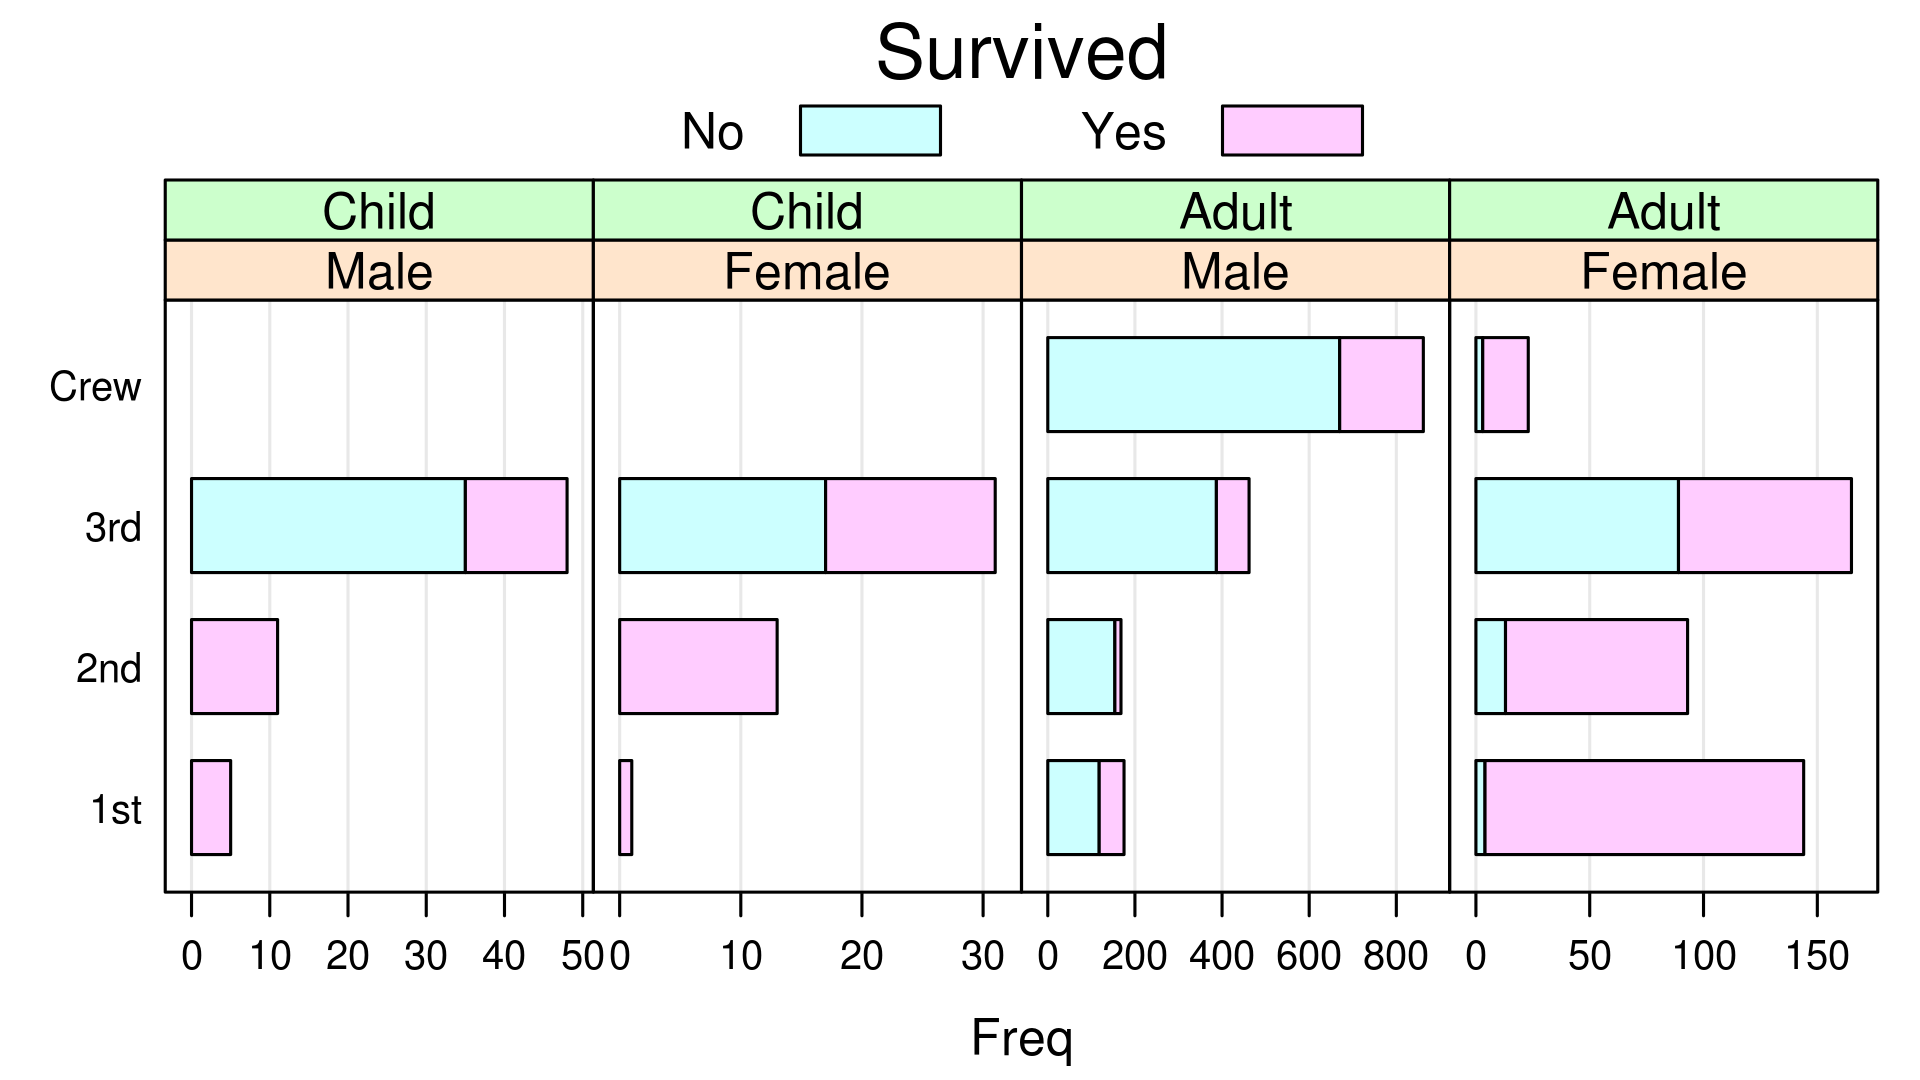
\includegraphics[width=0.7\columnwidth]{lattice-example2.png}
  \caption{泰坦尼克号生存率的交叉分类数据}
\end{figure}}
\end{overlayarea}  
\end{frame} 

\begin{frame}[t]{\subsecname}{公式参数}
\begin{itemize}
\item lattice的绘图函数都会\emphText{用公式作为第一位置参数}
\item<2-> 如果在不同panel中绘制多元数据,公式参数根据\emphText{“|”}符号后的变量对数据进行分类
\item<3-> 如果是在同一panel中绘制多元数据,则使用\emphText{group参数}对数据进行分类
\end{itemize}

\begin{overlayarea}{\textwidth}{\textheight}
\only<2>{
  \begin{table} \centering \footnotesize
    \begin{tabular}{|>{\centering\arraybackslash} m{0.2\columnwidth}|m{0.7\columnwidth}|}
      \toprule
      \rowcolor{LightCyan}
      \multicolumn{1}{|c|}{\textbf{公式参数}} & \multicolumn{1}{c|}{\textbf{含义}} \\\hline
      $\sim y$ & 单变量数据\\\hline
      $\sim y|z$ & 根据z变量对单变量数据划分panel\\\hline
      $y\sim x$ & 二元变量数据\\\hline
      $y\sim x|z $ & 根据z变量对二元变量数据划分panel\\\hline
      $y\sim x|a+b$ & 根据多条件变量划分panel,等价于$y\sim x|a$和$y\sim x|b$ \\\hline
      $y_1+y_2\sim x$ & 多元变量数据绘图,等价于$y_1\sim x$,和$y_2\sim x$\\\hline
      $z\sim x*y$ & 绘制三维图形(x,y,z)\\
      \bottomrule
    \end{tabular}
    \caption{lattice中的公式参数}
  \end{table}}
\end{overlayarea}
\end{frame} 

\begin{frame}[t,fragile]{\subsecname}{公式参数}
\begin{onlyenv}<1>
\begin{rcode}
> densityplot(|\colorbox{green}{$\sim$mpg}|, data=mtcars)
\end{rcode}
\begin{figure}
  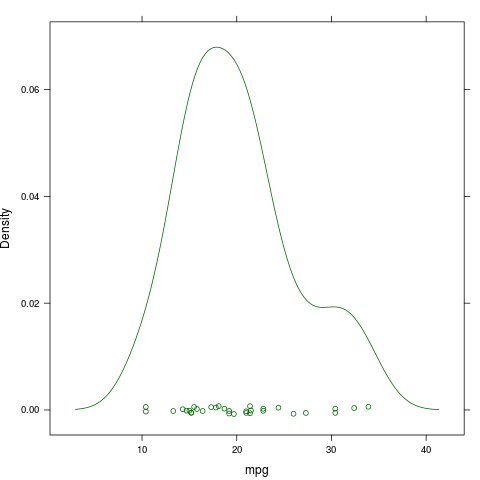
\includegraphics[width=0.6\columnwidth]{lattice-parameter1.png}
  \caption{在panel中绘制单变量数据}
\end{figure}
\end{onlyenv}

\begin{onlyenv}<2>
\begin{rcode}
> densityplot(|\colorbox{green}{$\sim$mpg\textbar cyl}|, data=mtcars, layout=c(1,3))
\end{rcode}
\begin{figure}
  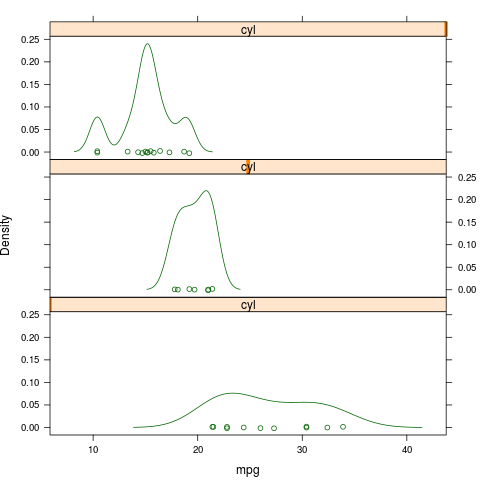
\includegraphics[width=0.6\columnwidth]{lattice-parameter2.png}
  \caption{在不同panel中绘制单变量分类数据}
\end{figure}
\end{onlyenv}

\begin{onlyenv}<3>
\begin{rcode}
> densityplot(~mpg, data=mtcars, |\colorbox{green}{group=cyl}|)
\end{rcode}
\begin{figure}
  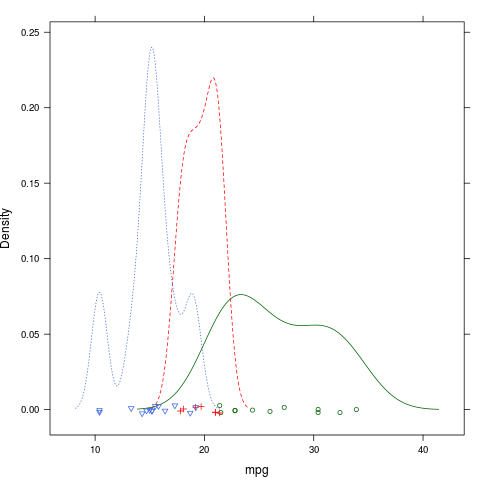
\includegraphics[width=0.6\columnwidth]{lattice-parameter3.png}
  \caption{在同一panel中绘制单变量分类数据}
\end{figure}
\end{onlyenv}

\begin{onlyenv}<4>
\begin{rcode}
> EE <- equal.count(ethanol$E, number=9, overlap=1/4)
> xyplot(|\colorbox{green}{NOx$\sim$ C \textbar EE}|, data = ethanol)
\end{rcode}
\begin{figure}
  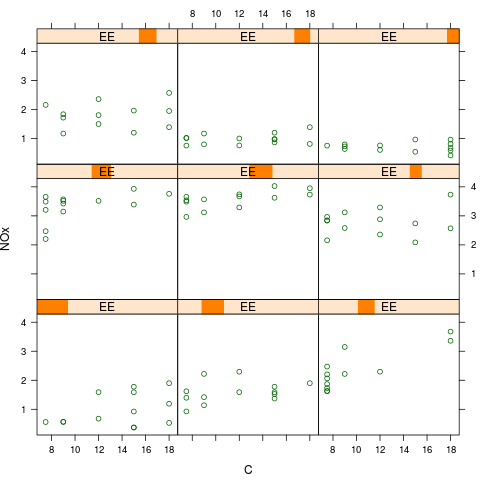
\includegraphics[width=0.6\columnwidth]{lattice-parameter4.png}
  \caption{在不同panel中绘制多变量分类数据}
\end{figure}
\end{onlyenv}
\end{frame} 

\begin{frame}[t]{\subsecname}{标准高级绘图函数}
\begin{itemize}
\item lattice包中提供了大量标准高级绘图函数用于直接绘制常用的统计图形
\end{itemize}
\vspace{-5pt}
\begin{figure}\centering
    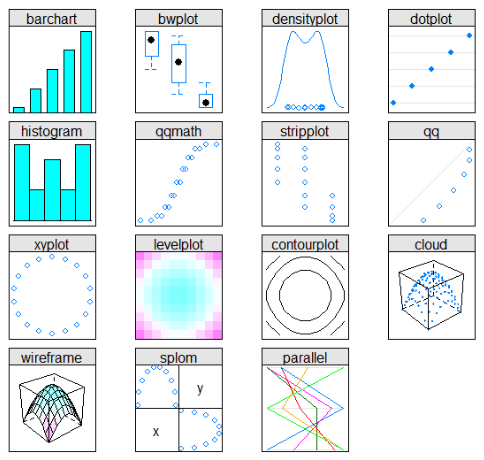
\includegraphics[width=0.6\columnwidth]{lattice-all.png}
    \caption{lattice中的标准高级绘图函数}
\end{figure}
\end{frame} 

\begin{frame}[t]{\subsecname}{标准高级绘图函数}
  \begin{table} \centering \scriptsize
    \begin{tabular}{|>{\centering\arraybackslash} m{0.2\columnwidth}|>{\centering\arraybackslash} m{0.2\columnwidth}|>{\centering\arraybackslash} m{0.2\columnwidth} |>{\centering\arraybackslash} m{0.2\columnwidth}|}
      \toprule
      \rowcolor{LightCyan}
      \multicolumn{1}{|c|}{\textbf{lattcie函数}} & \multicolumn{1}{c|}{\textbf{公式参数}} &
\multicolumn{1}{c|}{\textbf{描述}} & \multicolumn{1}{c|}{\textbf{graphics对应函数}} \\\hline
      barchart() & $y\sim x$ & 条形图 & barplot() \\\hline
      bwplot() & $y\sim x$ & 箱线图 & boxplot() \\\hline
      densityplot() & $\sim y$ & 核密度图 & plot.density()\\\hline
      dotplot() & $\sim y$ & Cleveland点图 & dotchart()\\\hline
      histogram() & $\sim x$ & 直方图 & hist()\\\hline
      stripplot() & $\sim y$ & 带状图 & stripchart()\\\hline
      xyplot() & $y\sim x$ & 散点图 & plot()\\\hline
      contourplot() & $z\sim x*y$ & 等高线图 & contour()\\\hline
      cloud() & $z\sim x*y$ &三维散点图 & 无\\\hline
      levelplot() & $z\sim x*y$ & 颜色图 & image()\\\hline
      wireframe() & $z\sim x*y$ & 三维透视图 & persp()\\\hline
      qq() & $\sim x$ & QQ图 & qqnorm()\\\hline
      splom() & $\sim data.frame$ & 散点图矩阵 & pairs()\\\hline
      parallel() & $\sim data.frame$ & 平行坐标图 & 无 \\
      \bottomrule
    \end{tabular}
    \caption{lattice包与graphics包的对应函数}
  \end{table}
\end{frame} 

\begin{frame}[t,fragile]{\subsecname}{panel函数和strip函数}
\begin{itemize}
\item lattice中每个高级绘图函数都有默认的panel参数和strip参数,
实质上对应的是两个匿名函数:\emphText{panel()和strip()}
\item 这两个函数可以用来对panel区域和strip区域需要绘制图形以及显示的
分类描述信息进行自定义扩展
%\item lattice也可以通过\emphText{update()}函数修改既有trellis对象中的绘图要素,从而达到修改图形的目的
\end{itemize}
\end{frame} 

\begin{frame}[c,fragile]{\subsecname}{panel函数和strip函数}
\begin{onlyenv}<1>
\begin{rcode}
# 在高级绘图函数中自定义panel和strip的示例
types.plain <- c("p", "l", "o", "r", "g", "s", "S", "h", "a", "smooth")
types.horiz <- c("s", "S", "h", "a", "smooth")
horiz <- rep(c(FALSE, TRUE), c(length(types.plain), length(types.horiz)))
types <- c(types.plain, types.horiz)
x <- sample(seq(-10, 10, length.out = 15), 30, TRUE)
y <- x + 0.25 * (x + 1)^2 + rnorm(length(x), sd = 5)

xyplot(y ~ x |\textbar| gl(1, length(types)),
       xlab = "type", 
       ylab = list(c("horizontal=TRUE", "horizontal=FALSE"), y = c(1/6, 4/6)), as.table = TRUE, layout = c(5, 3), between = list(y = c(0, 1)),
       # 自定义strip函数,...参数表示直接继承xyplot中的其他参数       
       |\colorbox{green}{strip = function(...)}|{
           # 调用标准panel函数panel.fill填充每个strip的颜色
           |\colorbox{green}{panel.fill}|(trellis.par.get("strip.background")$col[1])
           type <- types[panel.number()]
           # 调用底层grid绘图函数
           grid::grid.text(label = sprintf('"%s"', type), x = 0.5, y = 0.5)
           grid::grid.rect()
       },
       scales = list(alternating = c(0, 2), tck = c(0, 0.7), draw = FALSE),
       par.settings = list(layout.widths = list(strip.left = c(1, 0, 0, 0, 0))),
       # 自定义panel函数,...参数表示直接继承xyplot中的其他参数       
       |\colorbox{green}{panel = function(...)}| {
           type <- types[panel.number()]
           horizontal <- horiz[panel.number()]
           # 调用标准panel函数panel.xyplot按照预设参数每个panel中绘制图形  
           |\colorbox{green}{panel.xyplot}|(..., 
                        type = type,
                        horizontal = horizontal)
       })[rep(1, length(types))]
\end{rcode}
\end{onlyenv}

\begin{onlyenv}<2>
\begin{figure}\centering
    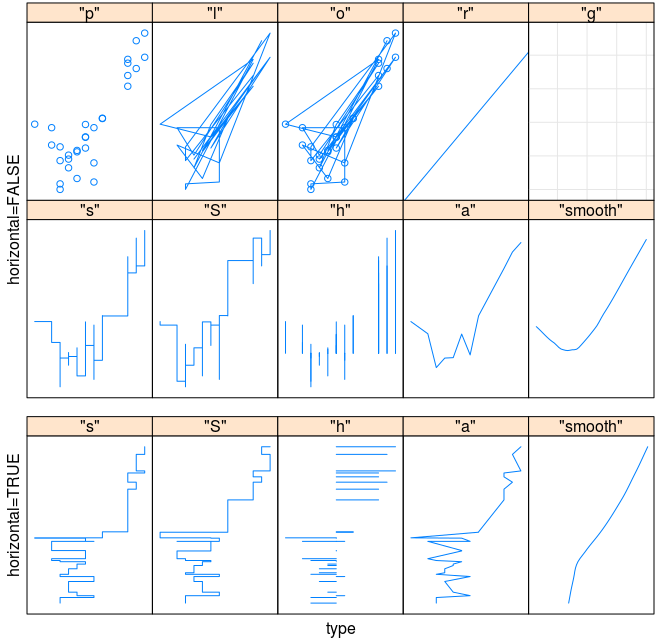
\includegraphics[width=0.7\columnwidth]{panel-example1.png}
    \caption{在高级绘图函数xyplot中自定义panel和strip}
\end{figure}
\end{onlyenv} 
\end{frame}

\begin{frame}[c,fragile]{\subsecname}{panel函数和strip函数}
\begin{figure}
 \begin{columns}
    \begin{column}[c]{.45\textwidth}
        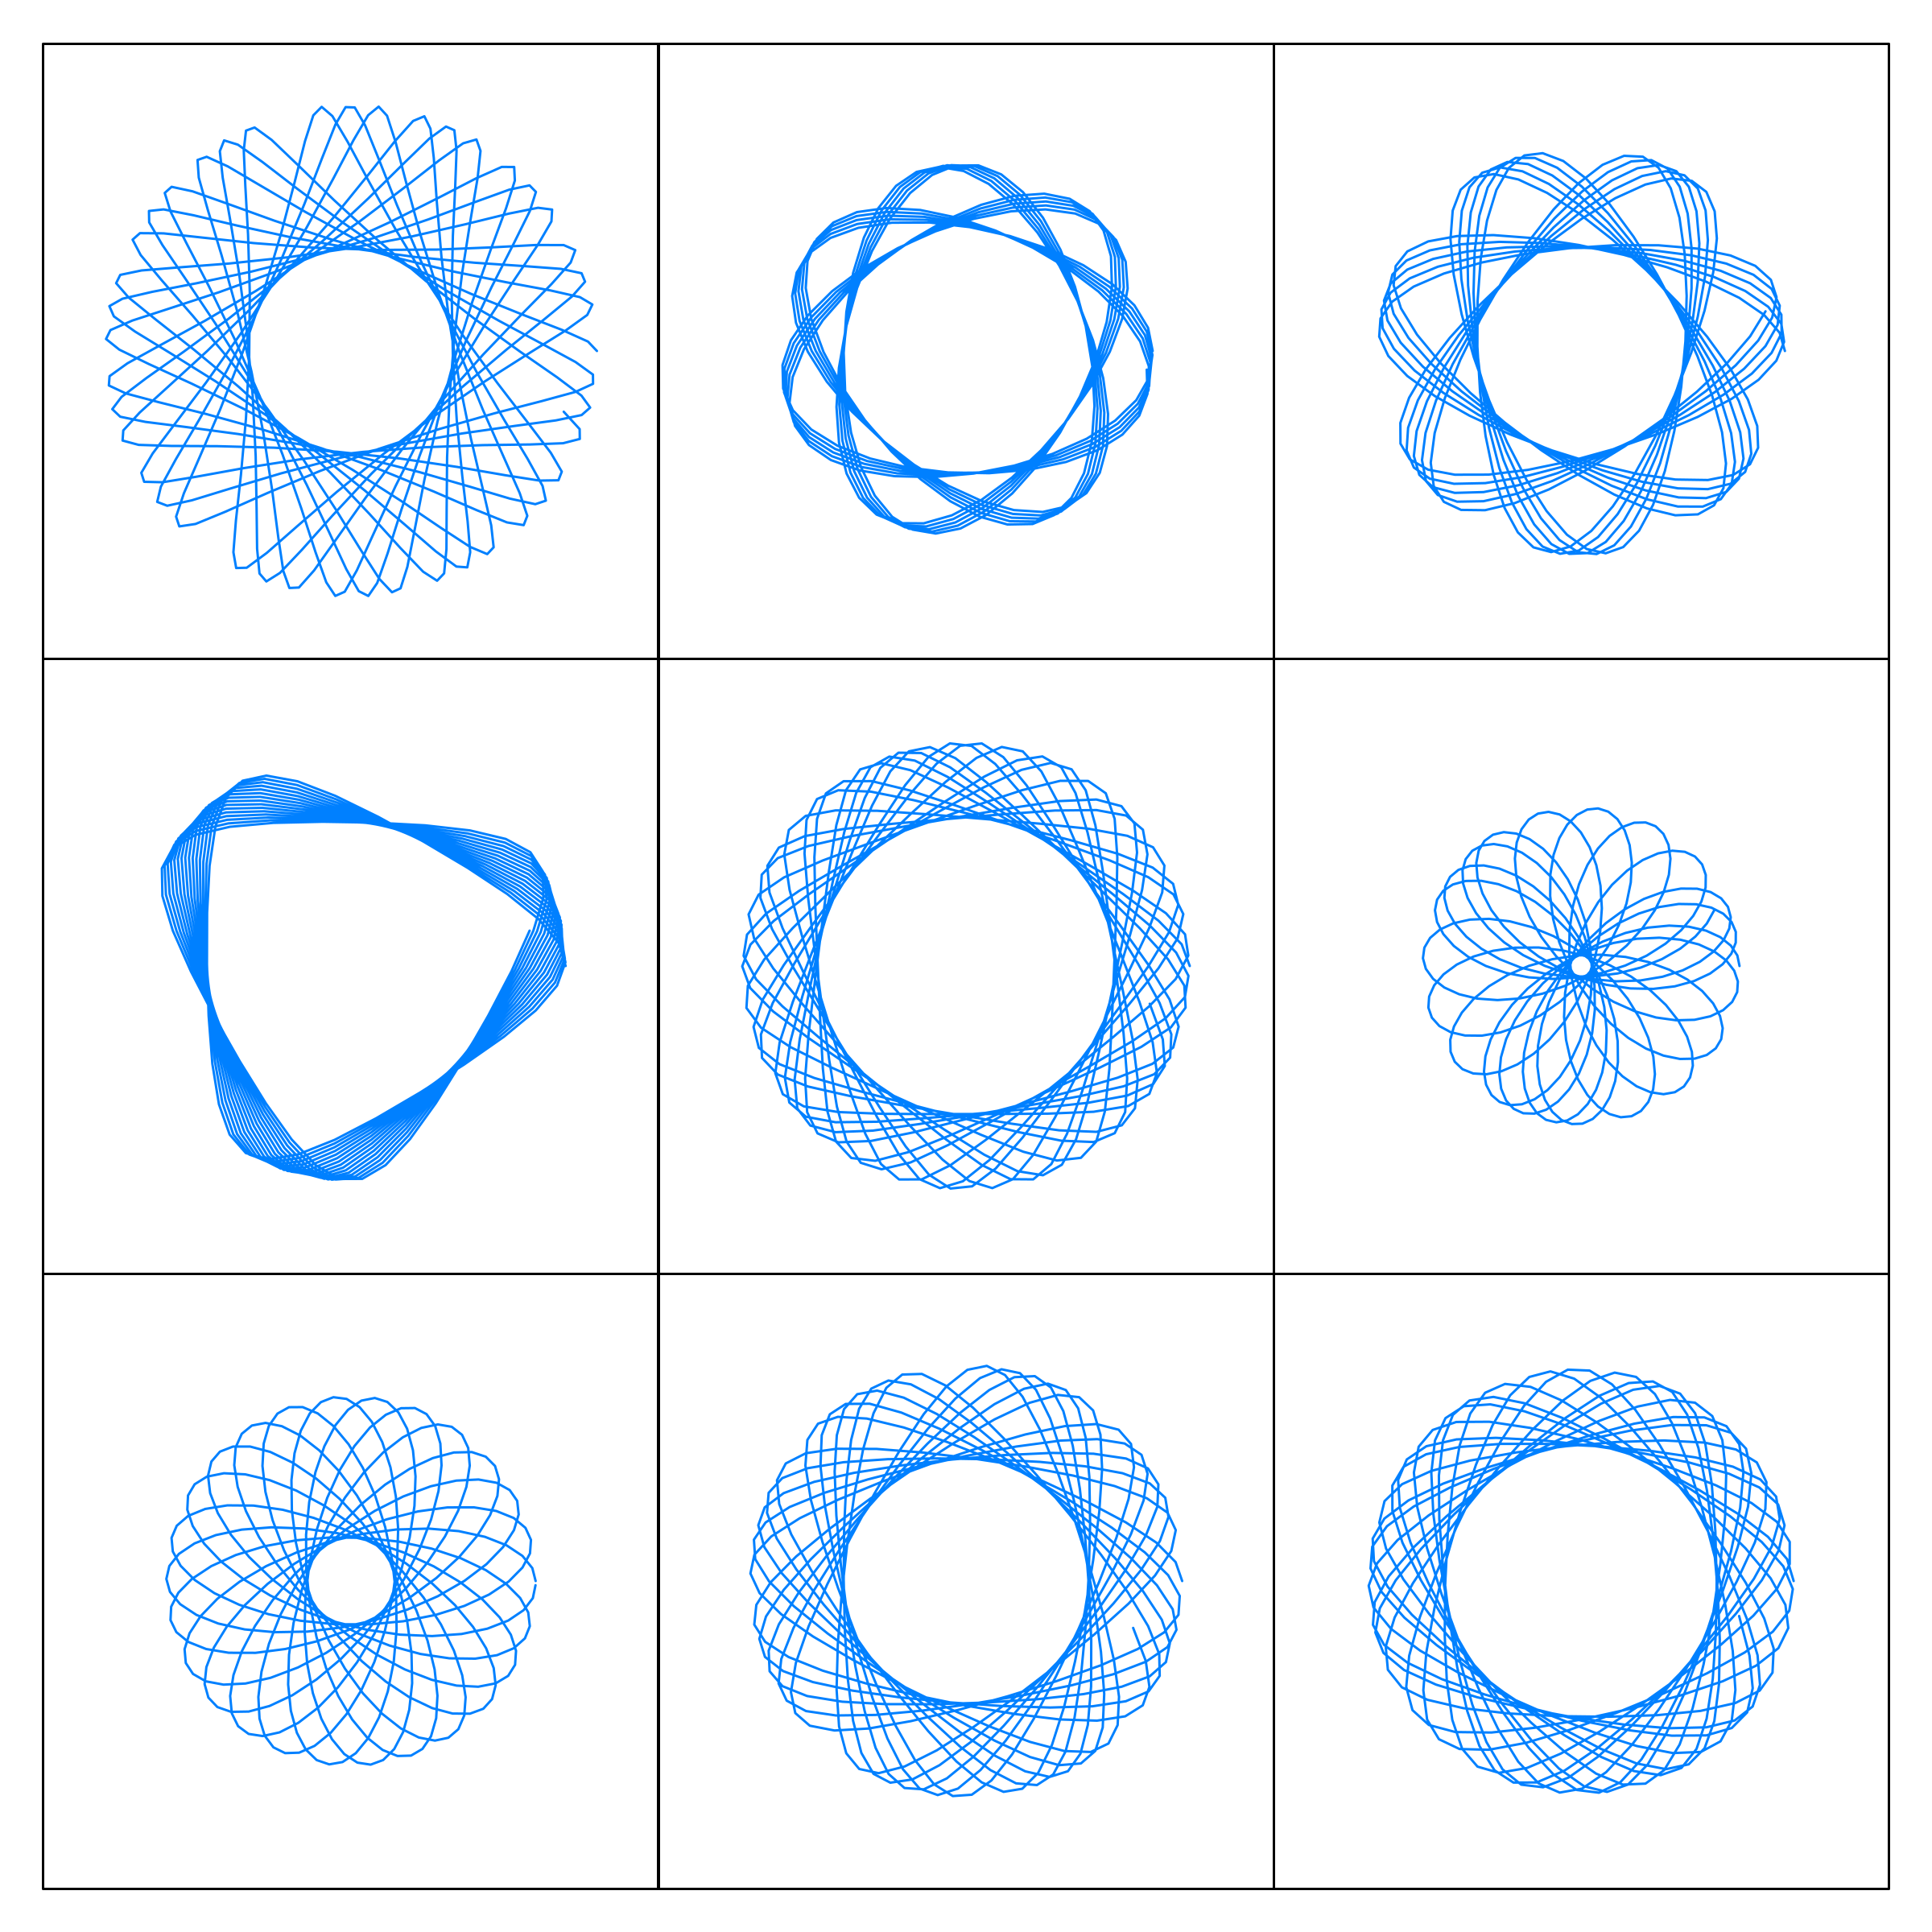
\includegraphics[width=\columnwidth]{panel-example2.png}
    \end{column}

    \begin{column}[c]{.55\textwidth}
\begin{rcode}
# 自定义一个panel函数绘制内旋轮线
# 注意:这个函数的所有参数都不是必选参数,而且没有...参数,这意味外部数据无法传入该函数参与绘图
> panel.hypotrochoid <- function(r, d, cycles = 10, density = 30)
 {
     if (missing(r)) r <- runif(1, 0.25, 0.75)
     if (missing(d)) d <- runif(1, 0.25 * r, r)
     t <- 2*pi*seq(0,cycles,by = 1/density)
     x <- (1-r)*cos(t)+d*cos((1-r)*t/r)
     y <- (1-r)*sin(t)-d*sin((1-r)*t/r)
     panel.lines(x, y)
 }
# 自定义prepanel函数来绘制panel的外框
> prepanel.hypocycloid <- function(x, y) {
     list(xlim=c(-1, 1),ylim = c(-1, 1))
 }

# 将xyplot函数传递给一个trellis对象p,这里传入的x参数其实并没有参与绘图
> p <- xyplot(x=c(-1, 1) ~ c(-1, 1), aspect = 1, cycles = 15, scales = list(draw = FALSE), xlab = "", ylab = "", panel = |\colorbox{green}{panel.hypotrochoid}|)
# 对象p循环绘图
> p[rep(1, 9)]
\end{rcode}
    \end{column}
  \end{columns}
  \caption{通过外部自定义panel函数来绘制图形}
\end{figure}
\end{frame} 

\begin{frame}[t,fragile]{\subsecname}{主题和图形参数设置}
\begin{itemize}
\item 在lattice中,所有的trellis对象都有一个主题(theme),theme中包含完整的图形要素:颜色、线宽、字体等
\item 当前theme的参数可以直接通过\emphText{trellis.par.get()}函数获取,通过
\emphText{trellis.par.set()}函数直接修改;\emphText{对theme参数的设置作用于当前绘图设备中的
所有高级绘图函数}
\end{itemize}
%\vspace{-10pt}

\begin{overlayarea}{\textwidth}{\textheight}
\begin{onlyenv}<1>
\begin{rcode}
# 罗列trellis对象中的所有图形参数
> names(trellis.par.get())
 [1] "grid.pars"         "fontsize"          "background"       
 [4] "panel.background"  "clip"              "add.line"         
 [7] "add.text"          "plot.polygon"      "box.dot"          
[10] "box.rectangle"     "box.umbrella"      "dot.line"         
[13] "dot.symbol"        "plot.line"         "plot.symbol"      
[16] "reference.line"    "strip.background"  "strip.shingle"    
[19] "strip.border"      "superpose.line"    "superpose.symbol" 
[22] "superpose.polygon" "regions"           "shade.colors"     
[25] "axis.line"         "axis.text"         "axis.components"  
[28] "layout.heights"    "layout.widths"     "box.3d"           
[31] "par.xlab.text"     "par.ylab.text"     "par.zlab.text"    
[34] "par.main.text"     "par.sub.text"    
\end{rcode}
\end{onlyenv}

\vspace{-10pt}
\begin{onlyenv}<2>
\begin{figure}[ht]
  \centering
  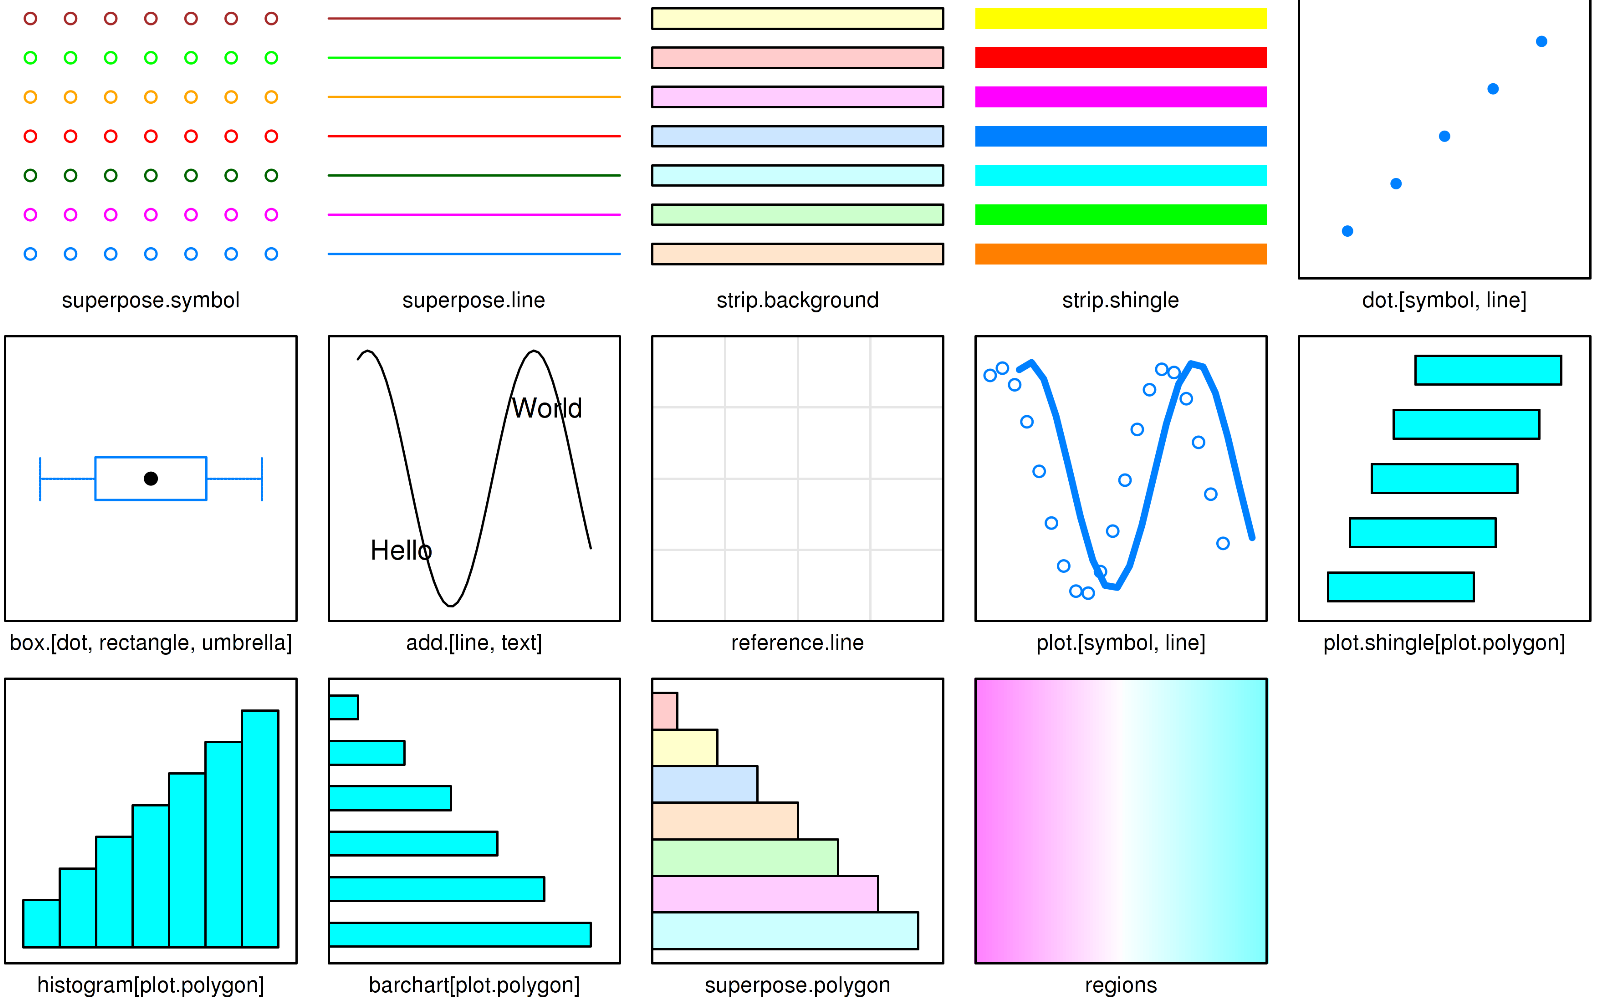
\includegraphics[width=0.7\columnwidth]{show_settings.png}
  \caption{trellis对象中所有的图形参数}
\end{figure}
\end{onlyenv}

\begin{onlyenv}<3>
\begin{figure}
 \begin{columns}
    \begin{column}[c]{.4\textwidth}
        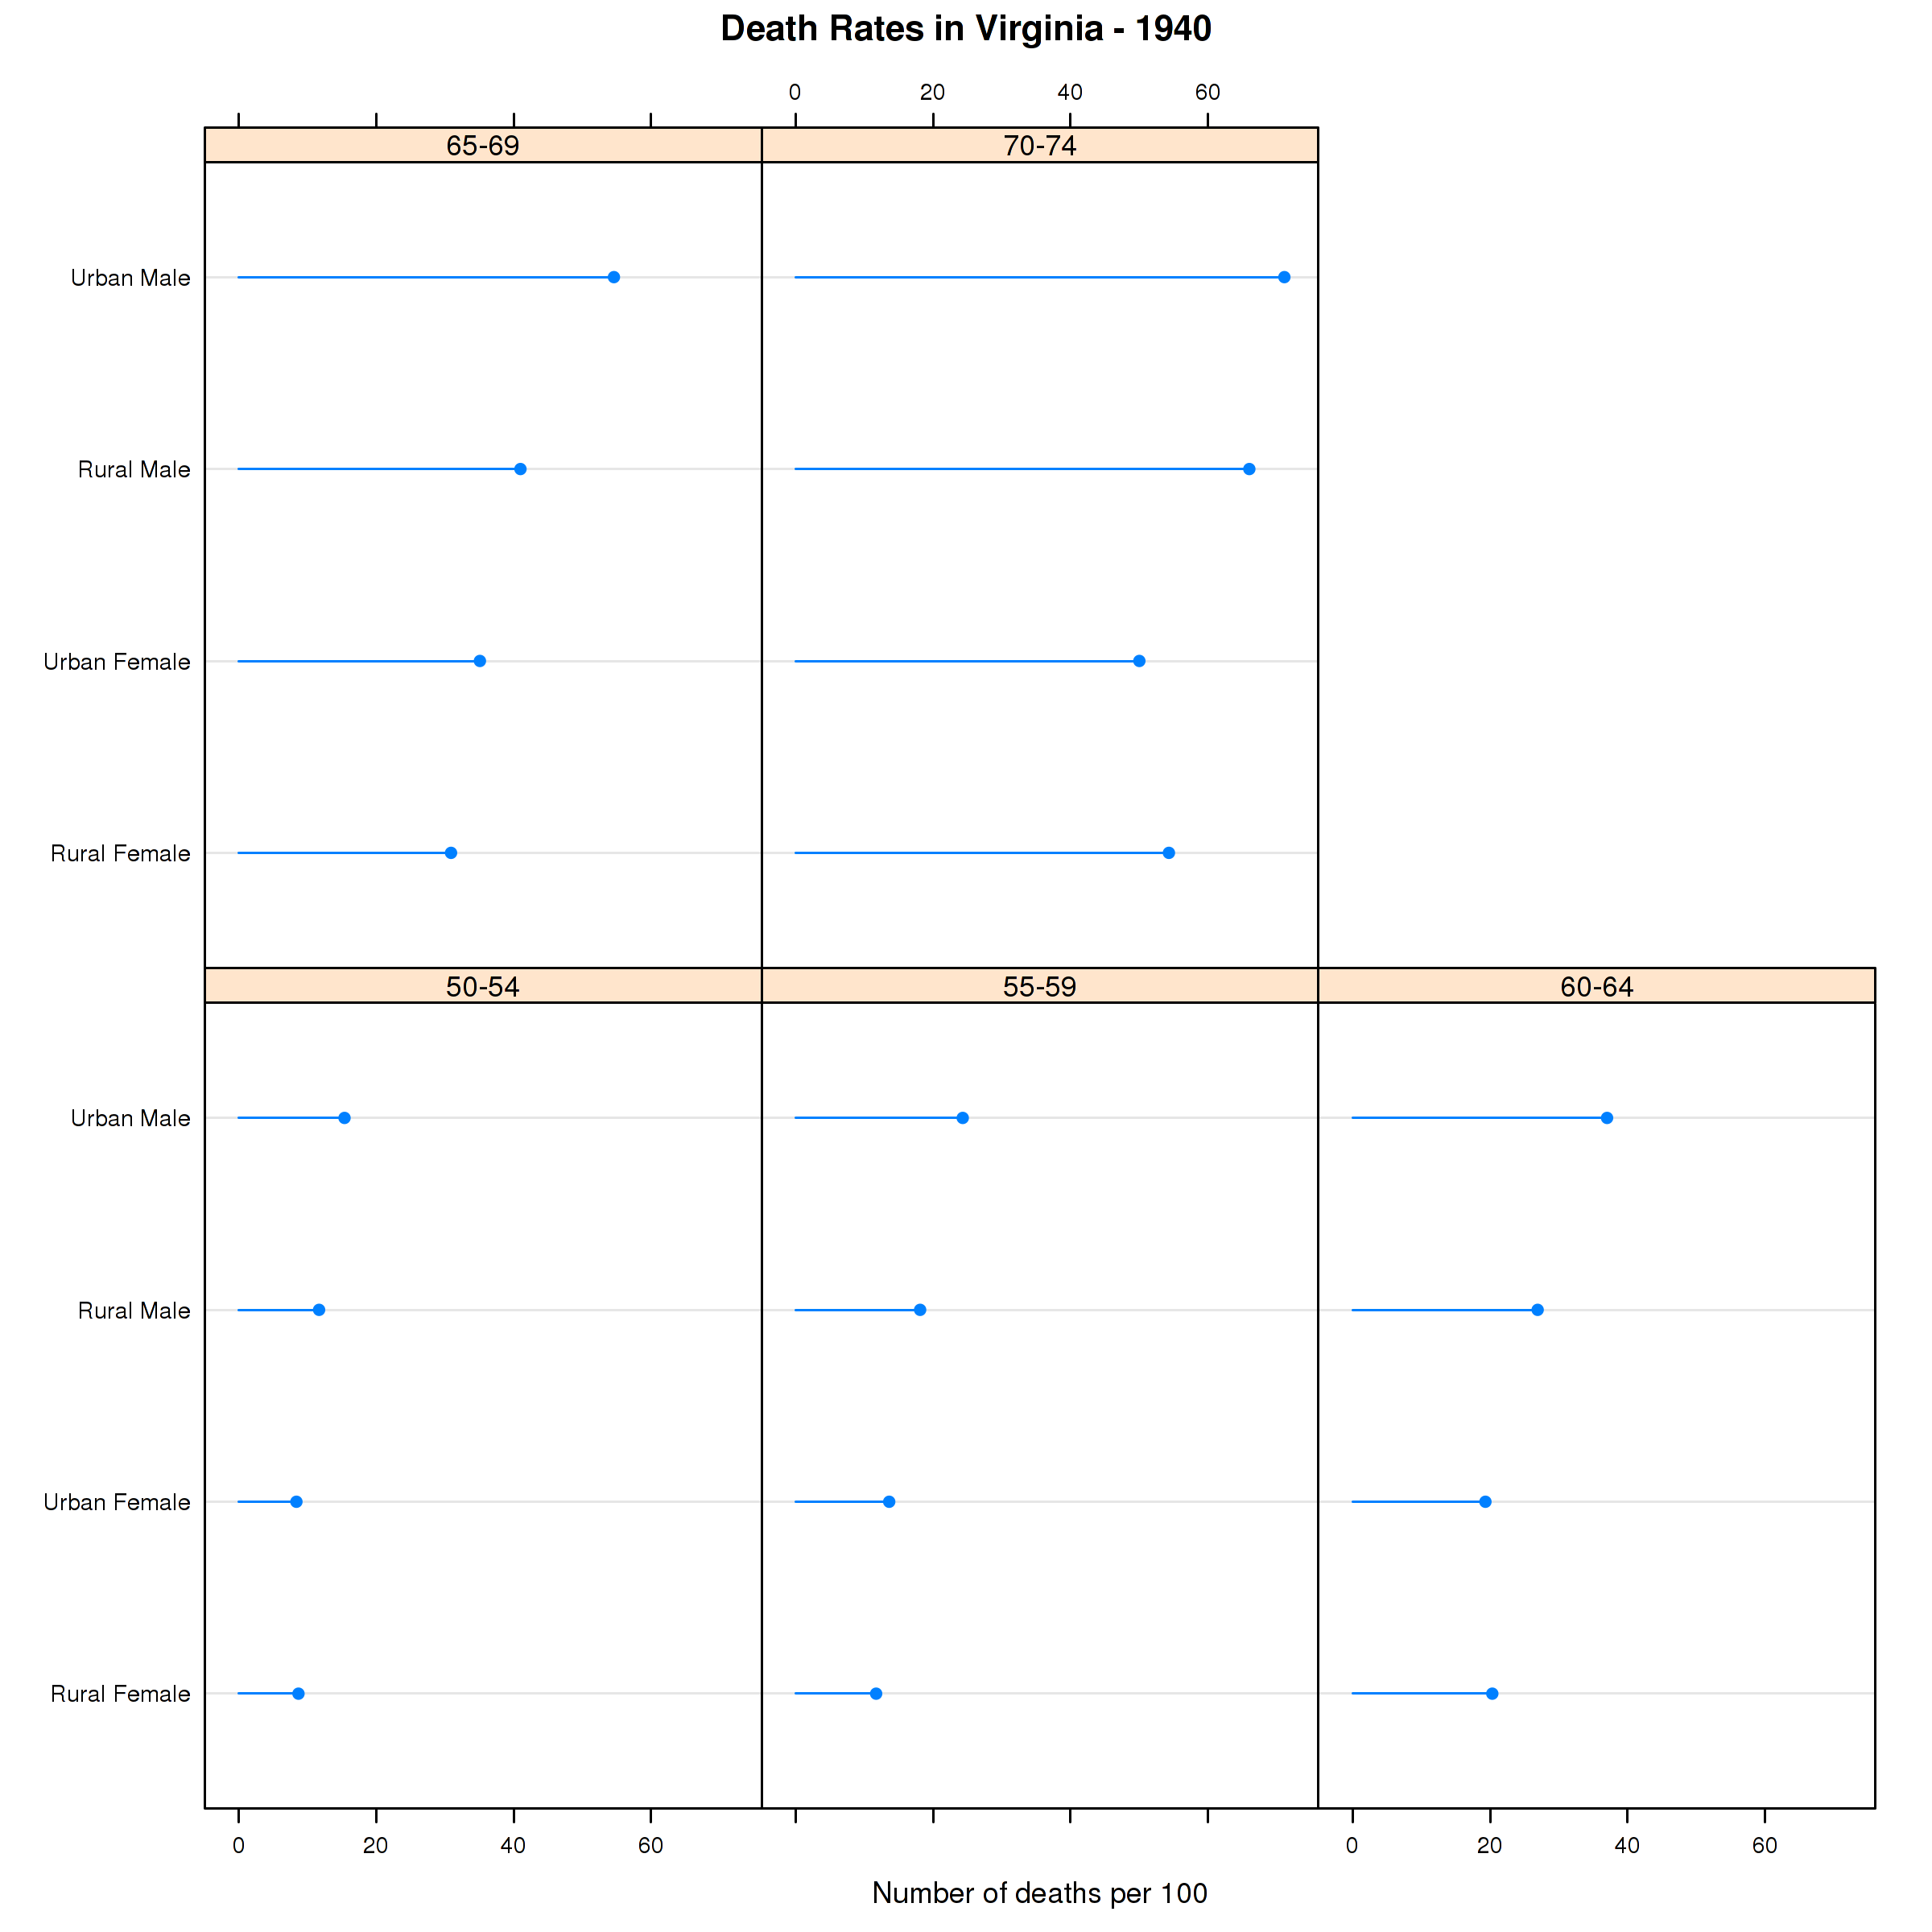
\includegraphics[width=\columnwidth]{trellis_par_set1.png}
    \end{column}

    \begin{column}[c]{.6\textwidth}
\begin{rcode}
# 绘制dotplot传递给trellis对象vad.plot
> vad.plot <- 
    dotplot(reorder(Var2, Freq)~Freq |\textbar| Var1,
            data = as.data.frame.table(VADeaths), 
            origin = 0, type = c("p", "h"),
            main = "Death Rates in Virginia - 1940", 
            xlab = "Number of deaths per 100")
> vad.plot
\end{rcode}
    \end{column}
  \end{columns}
  \caption{通过直接修改trellis对象的图形参数实现修改图形}
\end{figure}
\end{onlyenv}

%\vspace{-10pt}
\begin{onlyenv}<4>
\begin{figure}
 \begin{columns}
    \begin{column}[c]{.4\textwidth}
        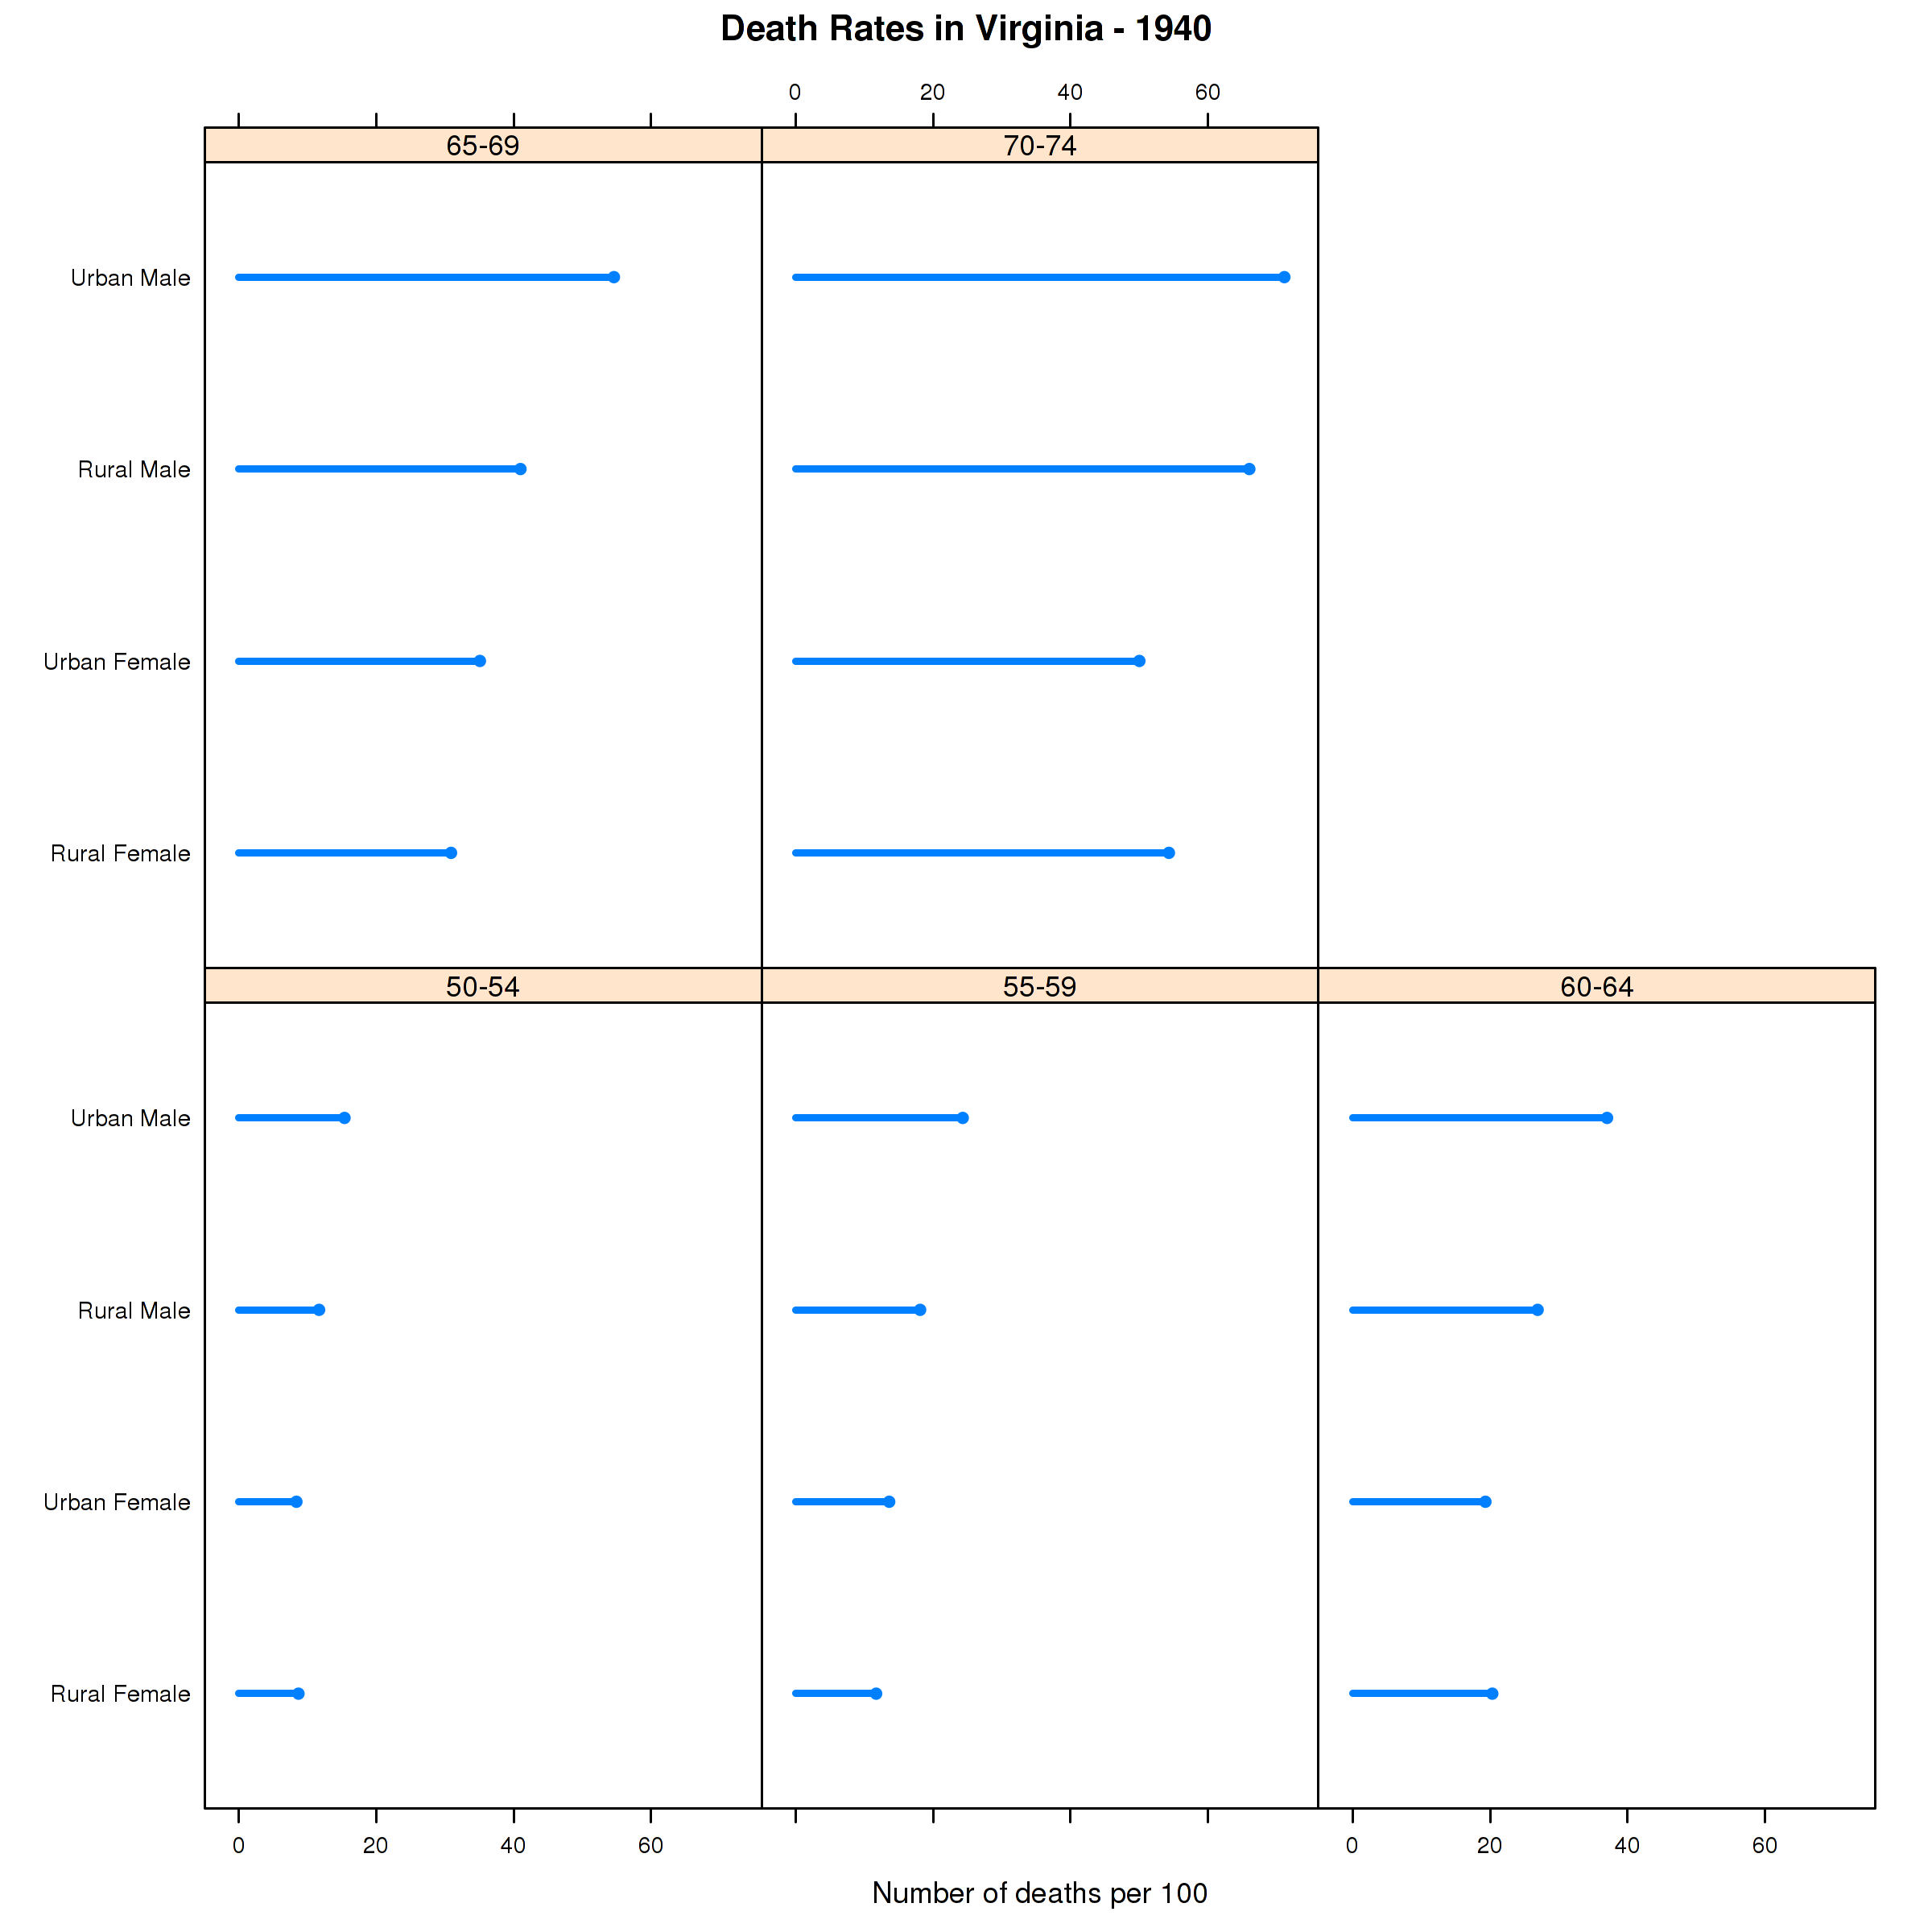
\includegraphics[width=\columnwidth]{trellis_par_set2.png}
    \end{column}

    \begin{column}[c]{.6\textwidth}
\begin{rcode}
# 在上图基础上修改绘图参数
# 获得当前主题的dot.line设置
> dot.line.settings <- |\colorbox{green}{trellis.par.get}|("dot.line")
# 将dot.line的颜色设置为透明不可见
> dot.line.settings$col <- "transparent"
# 应用新的参数设置
> |\colorbox{green}{trellis.par.set}|("dot.line", dot.line.settings)
# 获得当前主题的plot.line设置
> plot.line.settings <- |\colorbox{green}{trellis.par.get}|("plot.line")
# 将plot.line的线宽设置为3,默认是1
> plot.line.settings$lwd <- 3
# 应用新的参数设置
> |\colorbox{green}{trellis.par.set}|("plot.line", plot.line.settings)
> vad.plot
\end{rcode}
    \end{column}
  \end{columns}
  \caption{通过直接修改trellis对象的图形参数实现修改图形}
\end{figure}
\end{onlyenv}
\end{overlayarea}
\end{frame}

\begin{frame}[t,fragile]{\subsecname}{主题和图形参数设置}
\begin{itemize}
\item 除了设置theme参数之外,还可以通过\emphText{par.settings参数}仅对当前图形进行图形参数调整,
这比较类似par()函数的作用
\item 另外,lattice中提供了\emphText{update.trellis}函数来更新trellis对象的参数,
配合par.settings参数可以在不重绘图形的情况下实现图形的修改
\end{itemize}

\begin{overlayarea}{\textwidth}{\textheight}
\begin{onlyenv}<2>
\begin{figure}
 \begin{columns}
    \begin{column}[c]{.4\textwidth}
        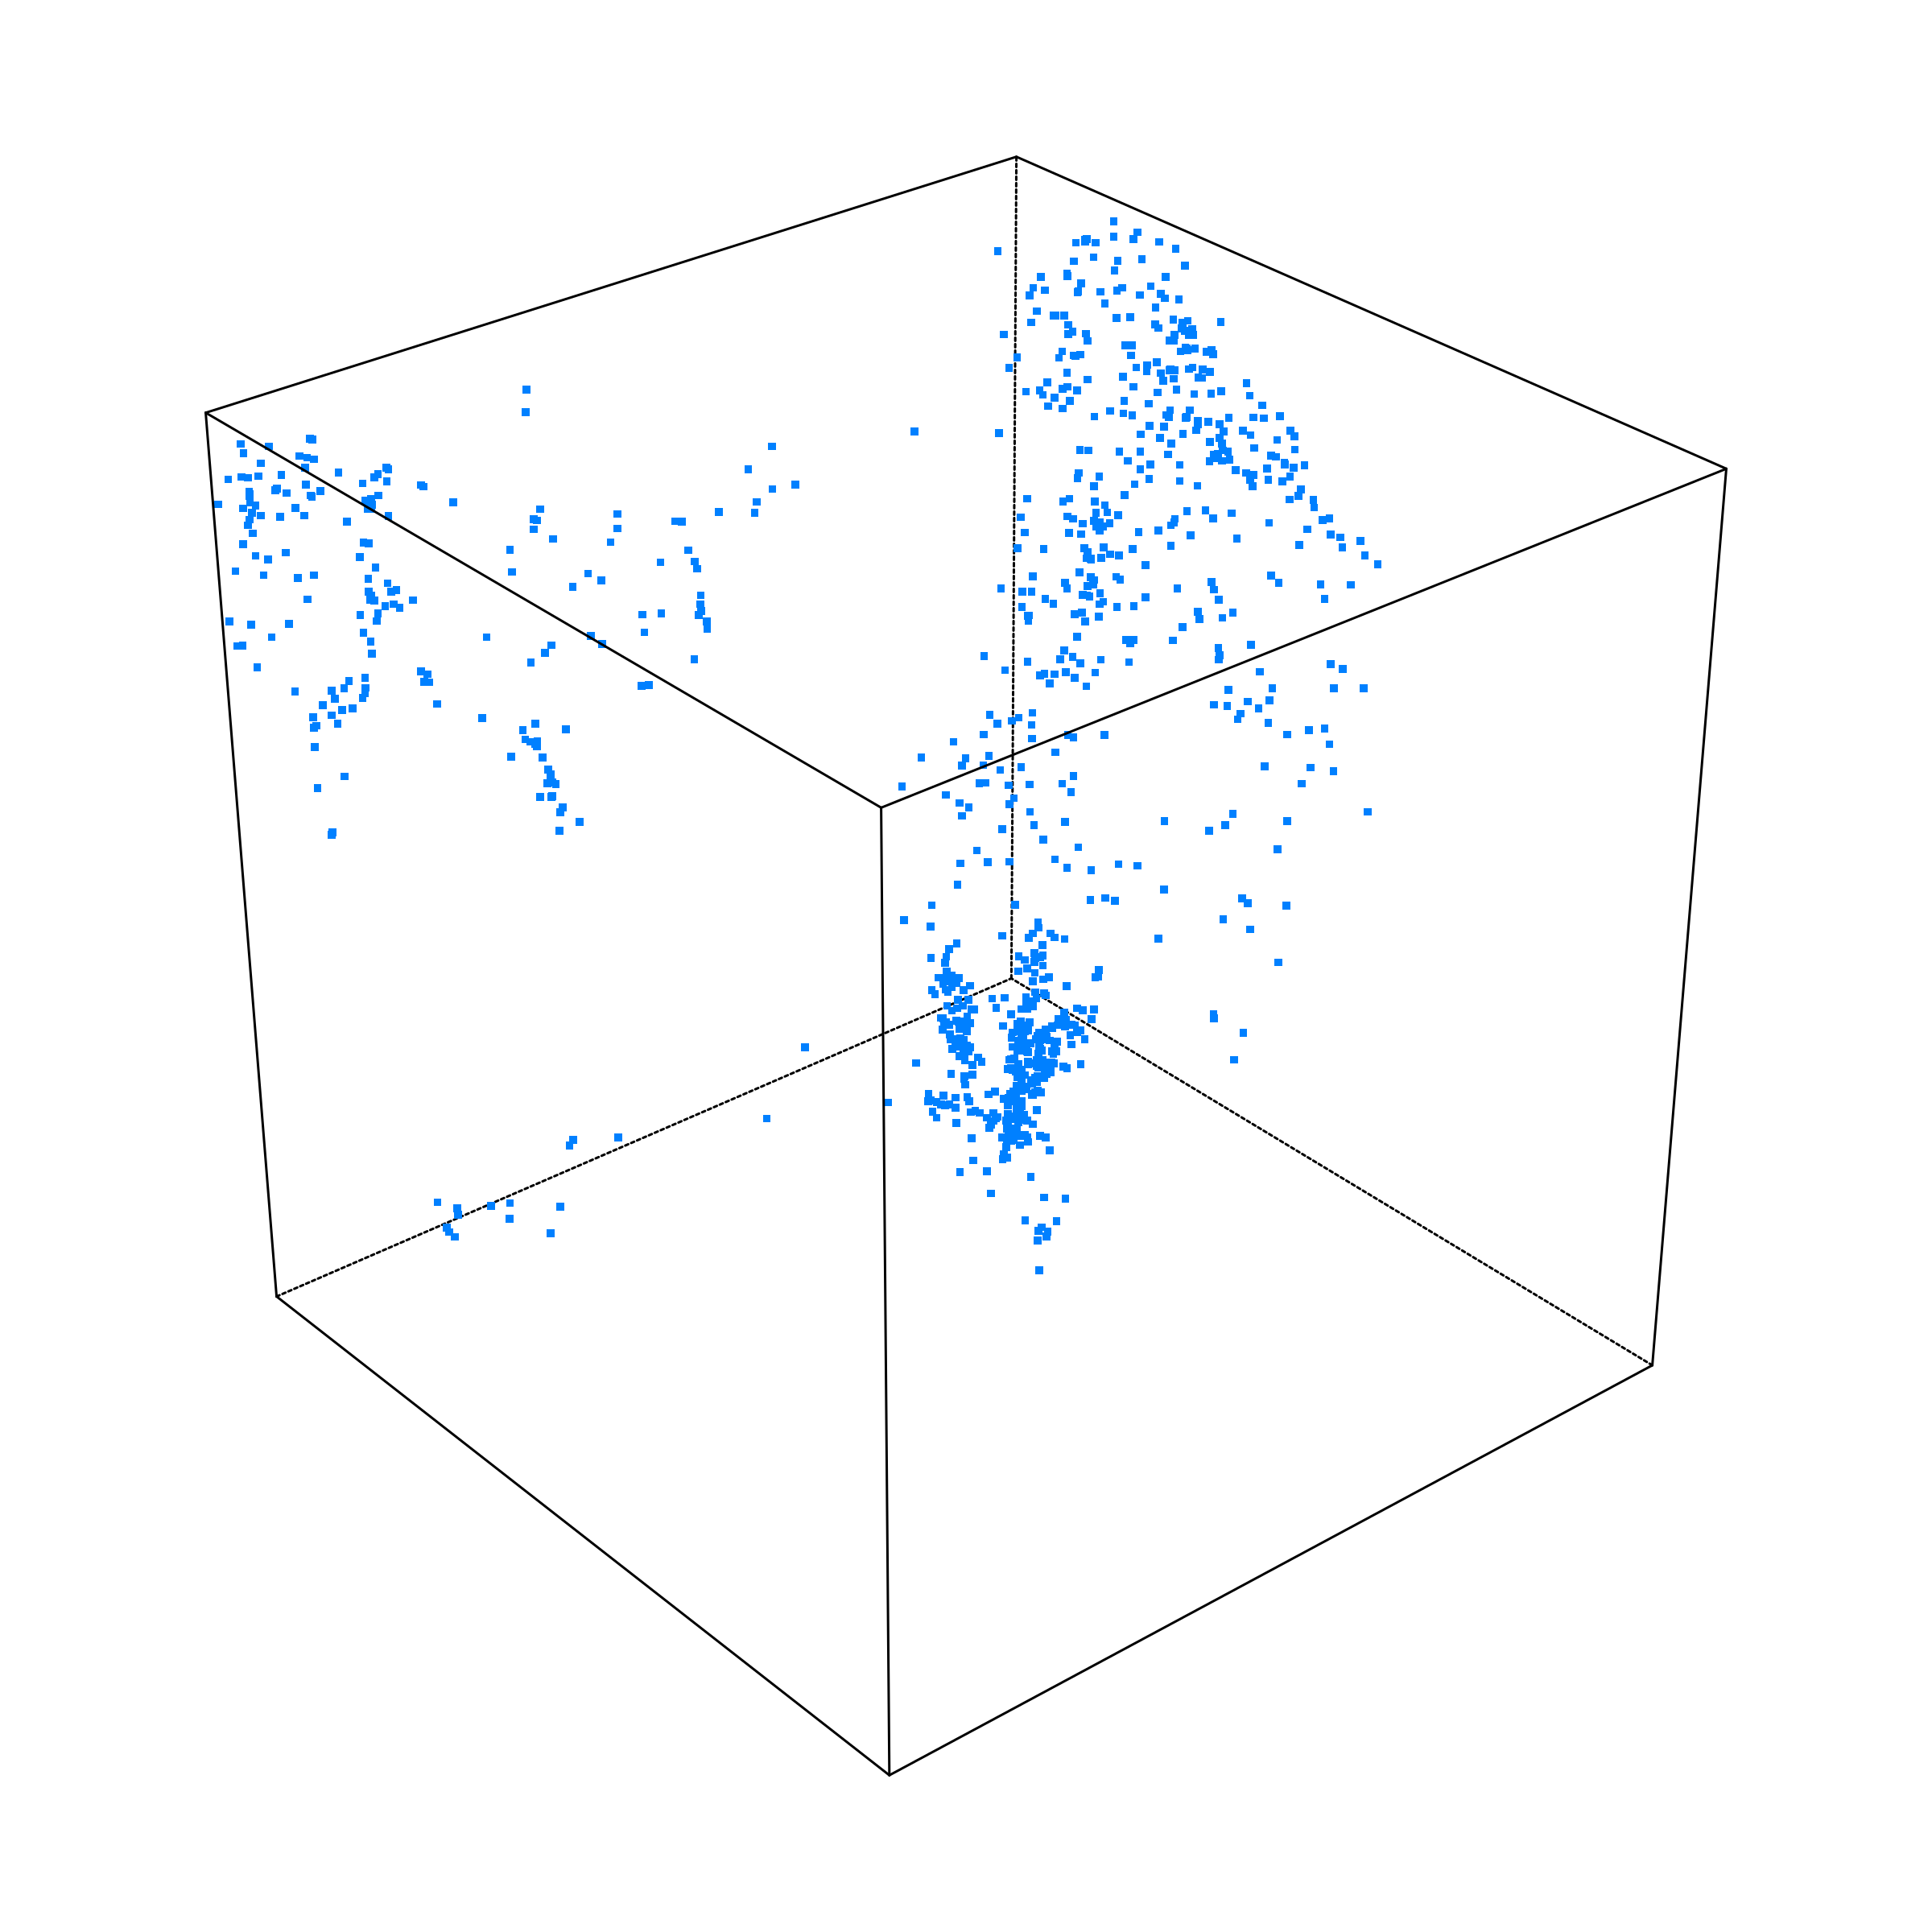
\includegraphics[width=\columnwidth]{update-example1.png}
    \end{column}

    \begin{column}[c]{.6\textwidth}
\begin{rcode}
# 首先定义一个三维散点图,并将其传入trellis对象p
> p <-
  cloud(depth ~ long + lat, quakes, zlim = c(690, 30), pch = ".", cex = 4, zoom = 1, xlab = NULL, ylab = NULL, zlab = NULL,scales = list(draw = FALSE),
        # 用par.settings参数设置坐标线为透明
        |\colorbox{green}{par.settings}|=list(axis.line = list(col = "transparent")))
> p
\end{rcode}
    \end{column}
  \end{columns}
  \caption{通过update函数和par.settings对象修改图形}
\end{figure}
\end{onlyenv}

\vspace{-10pt}
\begin{onlyenv}<3>
\begin{figure}
 \begin{columns}
    \begin{column}[c]{.4\textwidth}
        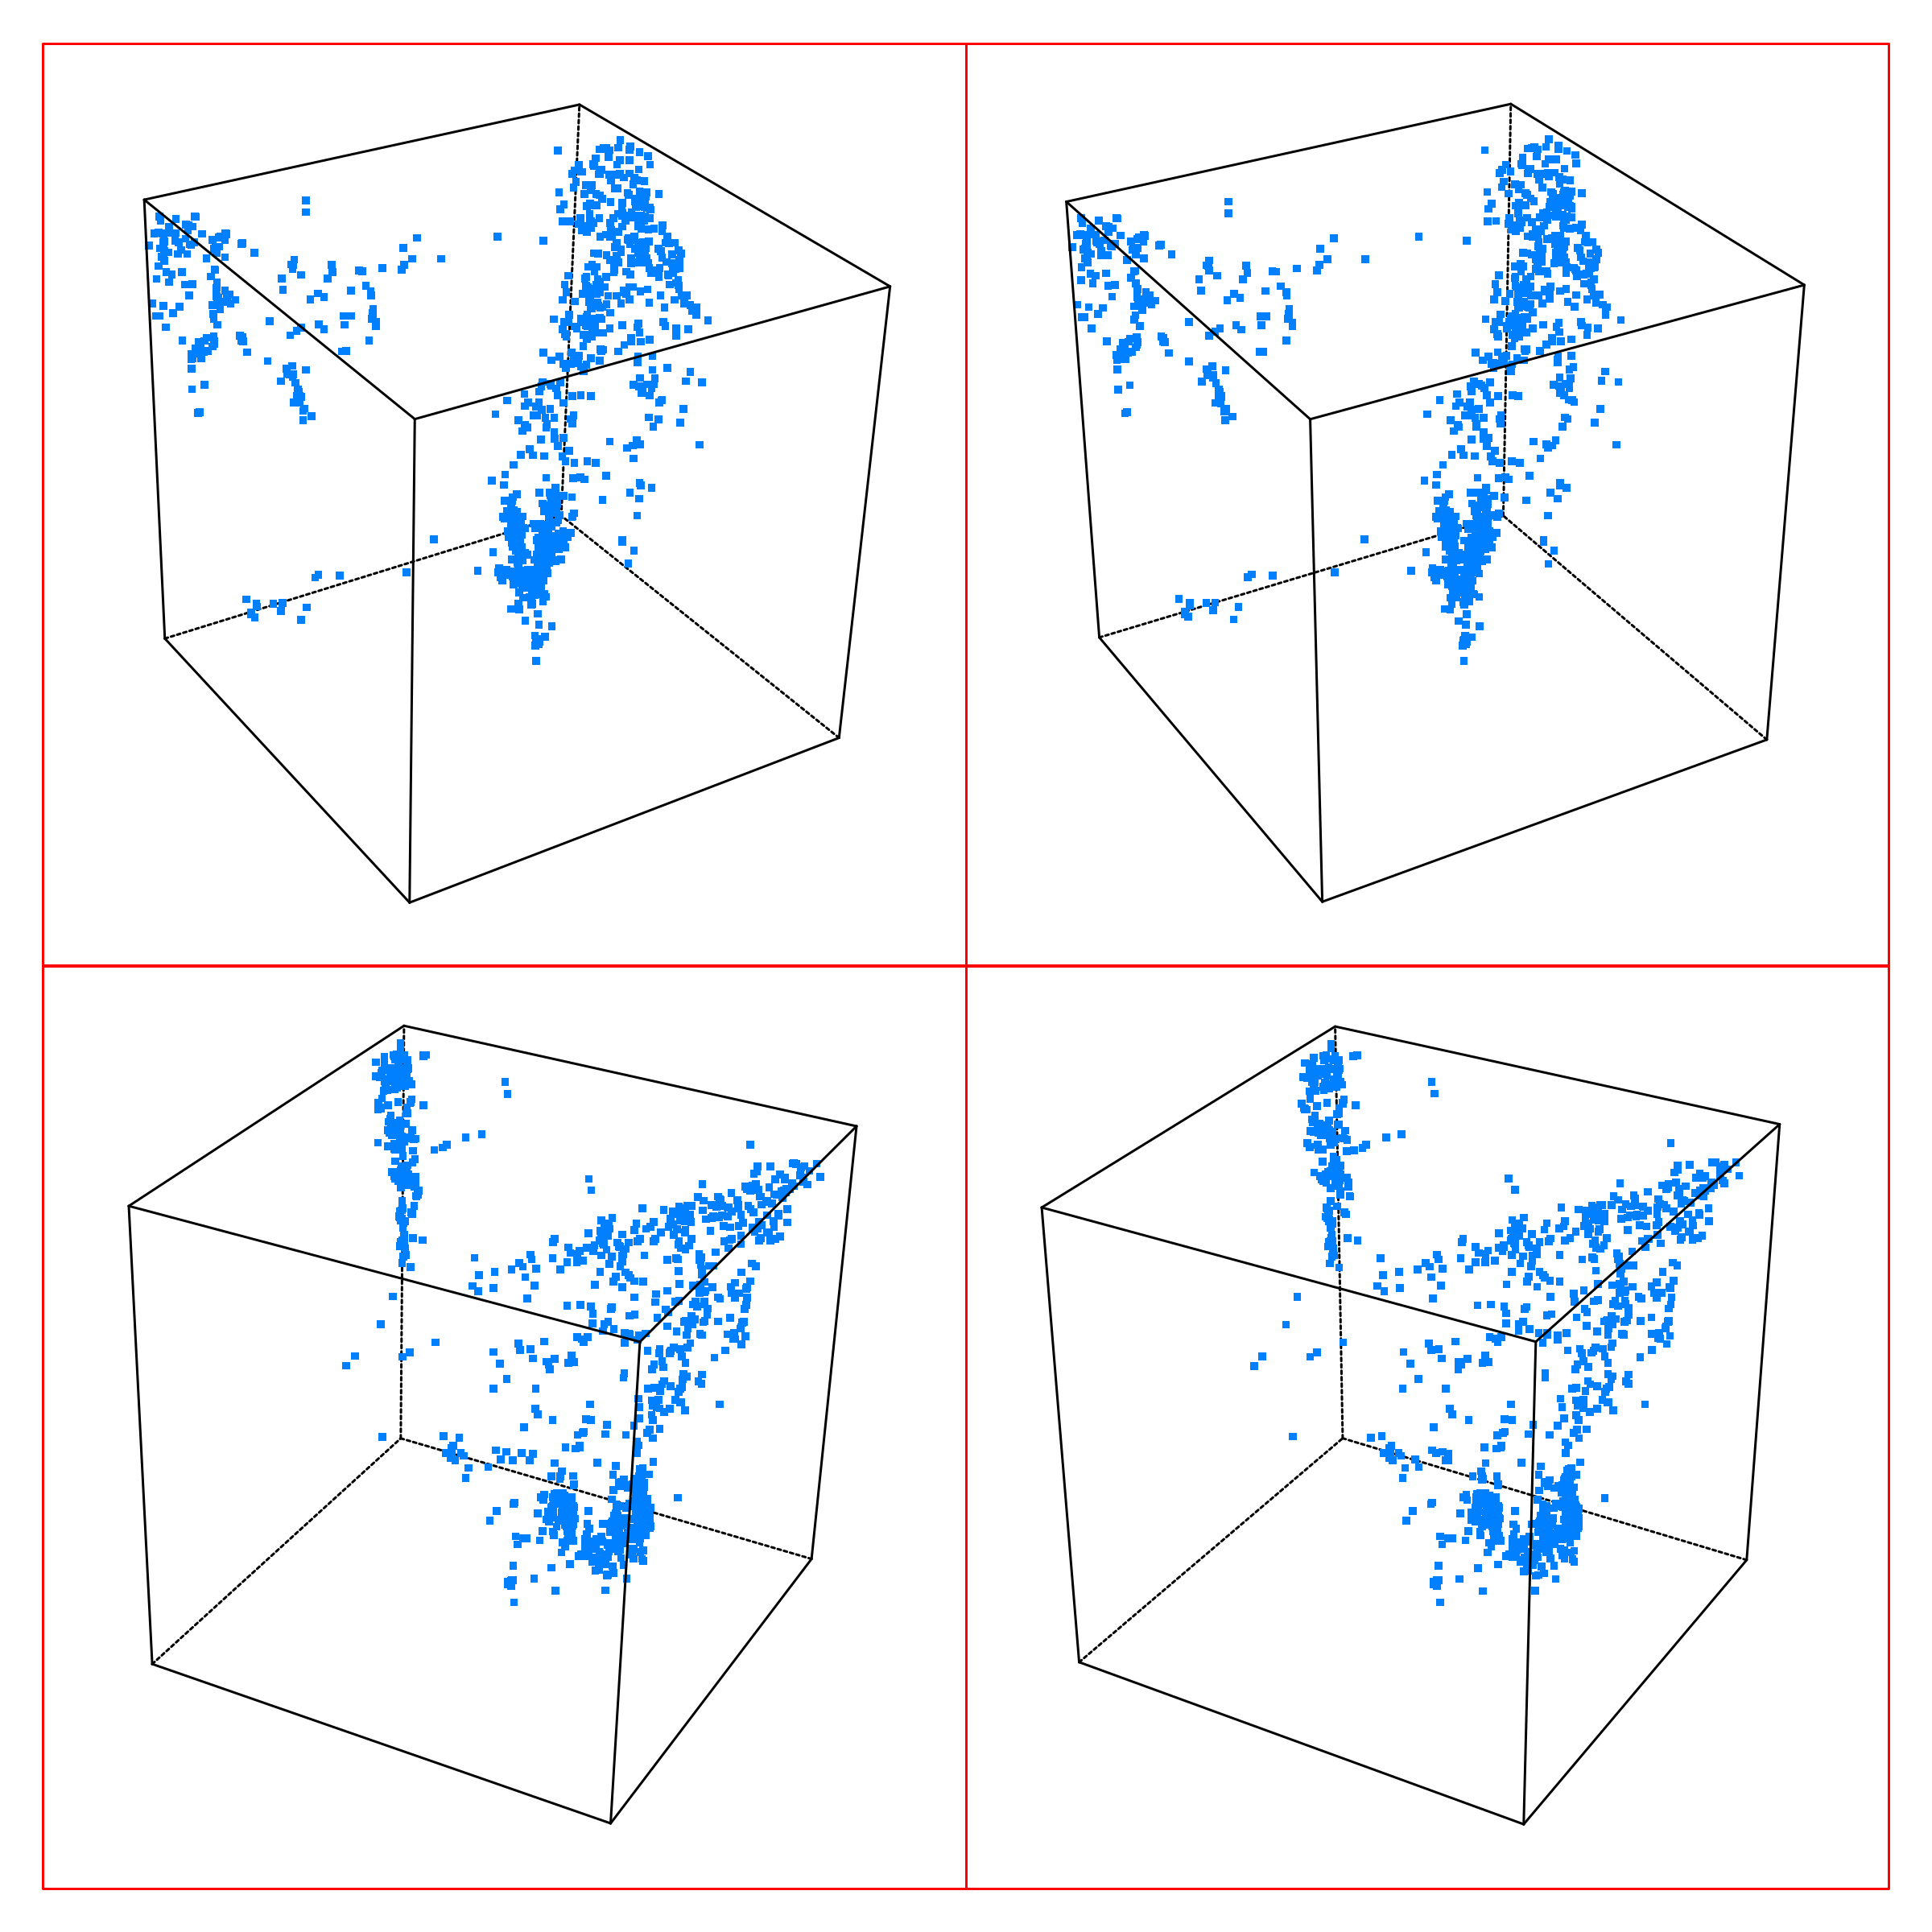
\includegraphics[width=\columnwidth]{update-example2.png}
    \end{column}

    \begin{column}[c]{.6\textwidth}
\begin{rcode}
> npanel <- 2
# 设置三维散点图的旋转视角
> rotz <- seq(-30, 30, length = npanel)
> roty <- c(3, 0)
# 用update.trellis函数更改原有图形
# 注意:由于update.trellis函数是一个继承自update函数的S3型对象,而传入的p是trellis对象,因此这里直接可以写update
> |\colorbox{green}{update}|(p[rep(1, 2 * npanel)], 
         layout = c(2, npanel),
         panel = function(..., screen) {
           crow <- current.row()
           ccol <- current.column()
         panel.cloud(..., screen = list(z = rotz[crow], x = -60, y = roty[ccol]))},
         # 用par.settings参数设置坐标线颜色为红 
         |\colorbox{green}{par.settings}|=list(axis.line=list(col="red")))
\end{rcode}
    \end{column}
  \end{columns}
  \caption{通过trellis对象的图形参数实现修改图形}
\end{figure}
\end{onlyenv}
\end{overlayarea}
\end{frame}

%%%https://www.cnblogs.com/nxld/p/6059603.html
%%%https://www.zhihu.com/question/24779017

\subsection{ggplot2程序包}
\begin{frame}[t]{\subsecname}{}
\begin{itemize}
\item ggplot2是grid绘图系统的另一个广泛使用的实现包,由\href{http://hadley.nz/}{\uline{Hadley Wickham}}开发维护,\emphText{目前该包尚未纳入base包,需要单独下载} 
\end{itemize}
\begin{figure}[ht]
  \centering
  
\includegraphics[width=0.9\columnwidth]{hadley_wickham.png}
  \caption{ggplot2程序包的作者Hadley Wickham(简称H.W.).他是R领域最知名的开发者之一,贡献了许多
重要的基础程序包,推进了R在世界上的广泛应用;目前担任RStudio公司首席科学家一职}
\end{figure}
\end{frame}

\begin{frame}[t]{\subsecname}{}
\begin{itemize}
\item ggplot2的设计理念来自Leland Wilkinson的\emphText{《The Grammar of Graphics》}一书,其吸取了书中提出的绘图理论和优雅的绘图语法:\emphText{将绘图与数据分离,数据相关绘图与数据无关绘图分离}
\end{itemize}
\begin{figure}[ht]
  \centering
  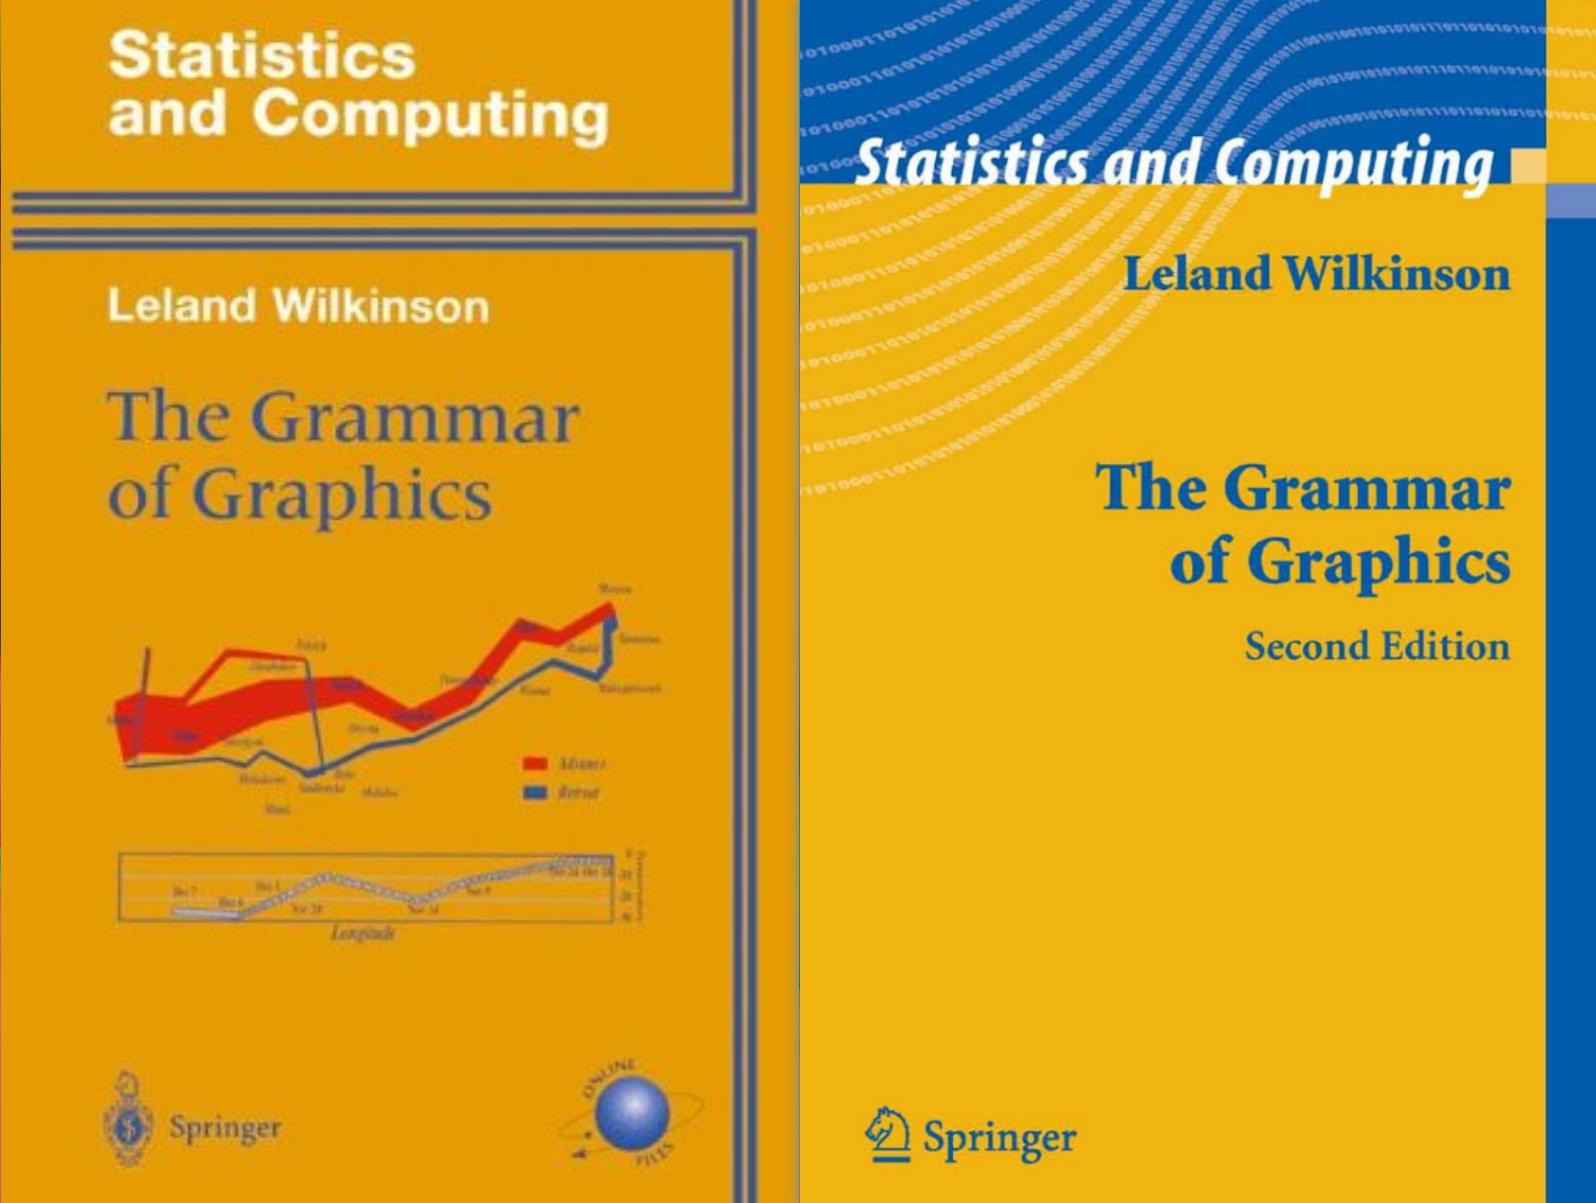
\includegraphics[width=0.65\columnwidth]{the_grammar_of_graphics.png}
  \caption{统计图形领域经典著作《The Grammar of Graphics》的第一版(1999)和第二版(2005),ggplot2的命名就取自这本书的首字母缩写再加上plot}
\end{figure}
\end{frame}

\begin{frame}[t,fragile]{\subsecname}{绘图原理}
\begin{itemize}
\item<1-> 将绘图与数据分离,数据相关绘图与数据无关绘图分离
\item<2-> 按照\emphText{图层(layer)}概念绘图,图层之间的叠加通过“+”符号实现,越往后的图层越在上层
\item<2-> 有明确的起始(ggplot函数)与终止,\emphText{一条语句绘制一张图}
\item<3-> 和lattice包一样,所有绘图内容都保存在\emphText{一个绘图对象}中
\item<4-> 保留标准绘图系统的\emphText{命令式调整函数},对图形做微调
\item<4-> 将\emphText{统计变换}设计成绘图过程中必不可少的步骤
\end{itemize}

\begin{overlayarea}{\textwidth}{\textheight}
\begin{onlyenv}<5>
\begin{minipage}{\textwidth}
\begin{rcode}
# graphics中的实现
# 以plot开始,可以以任何方式结束,每加上一个元素,实际上都是一句单独的命令,这与人类对于画图的认识有冲突,而且由于没有停止绘图的标志,使得后续操作会产生困惑
> x <- rnorm(100,10,5)
> y <- x + rnorm(100,0,1)
> plot(x,y)   #绘制散点图
> text(15,20, expression(x[1] == x[2])) #添加注释
\end{rcode} 
\end{minipage}

\begin{minipage}{\textwidth}
\begin{rcode}
# ggplot2中的实现
# 1、有明确的起始(以ggplot函数开始)与终止(一句语句一幅图)
# 2、图层之间的叠加是靠“+”号实现的,越往后的图层越高
> x <- rnorm(100,10,5) 
> y <- x + rnorm(100,0,1) 
> |\colorbox{green}{ggplot}|(data = NULL, aes(x = x, y = y)) +  #开始绘图
  |\colorbox{green}{geom\_point}|(color = "darkred") +  #添加点
  |\colorbox{green}{annotate}|("text",x = 15, y = 20,parse = T,label = "x[1]==x[2]") #添加注释
\end{rcode}
\end{minipage}
\end{onlyenv}
\end{overlayarea}
\end{frame}

\begin{frame}[t,fragile]{\subsecname}{数据无关的图形要素}
\begin{itemize}
\item 数据无关的图形要素\emphText{负责实现图形的结构化外观}
\item 通过\emphText{theme()}函数对数据无关的图形要素进行统一设置,包括四个基础类型:文本、线、矩形和空白
\end{itemize}

\begin{overlayarea}{\textwidth}{\textheight}
\only<1>{
\begin{figure}[ht]
  \centering
  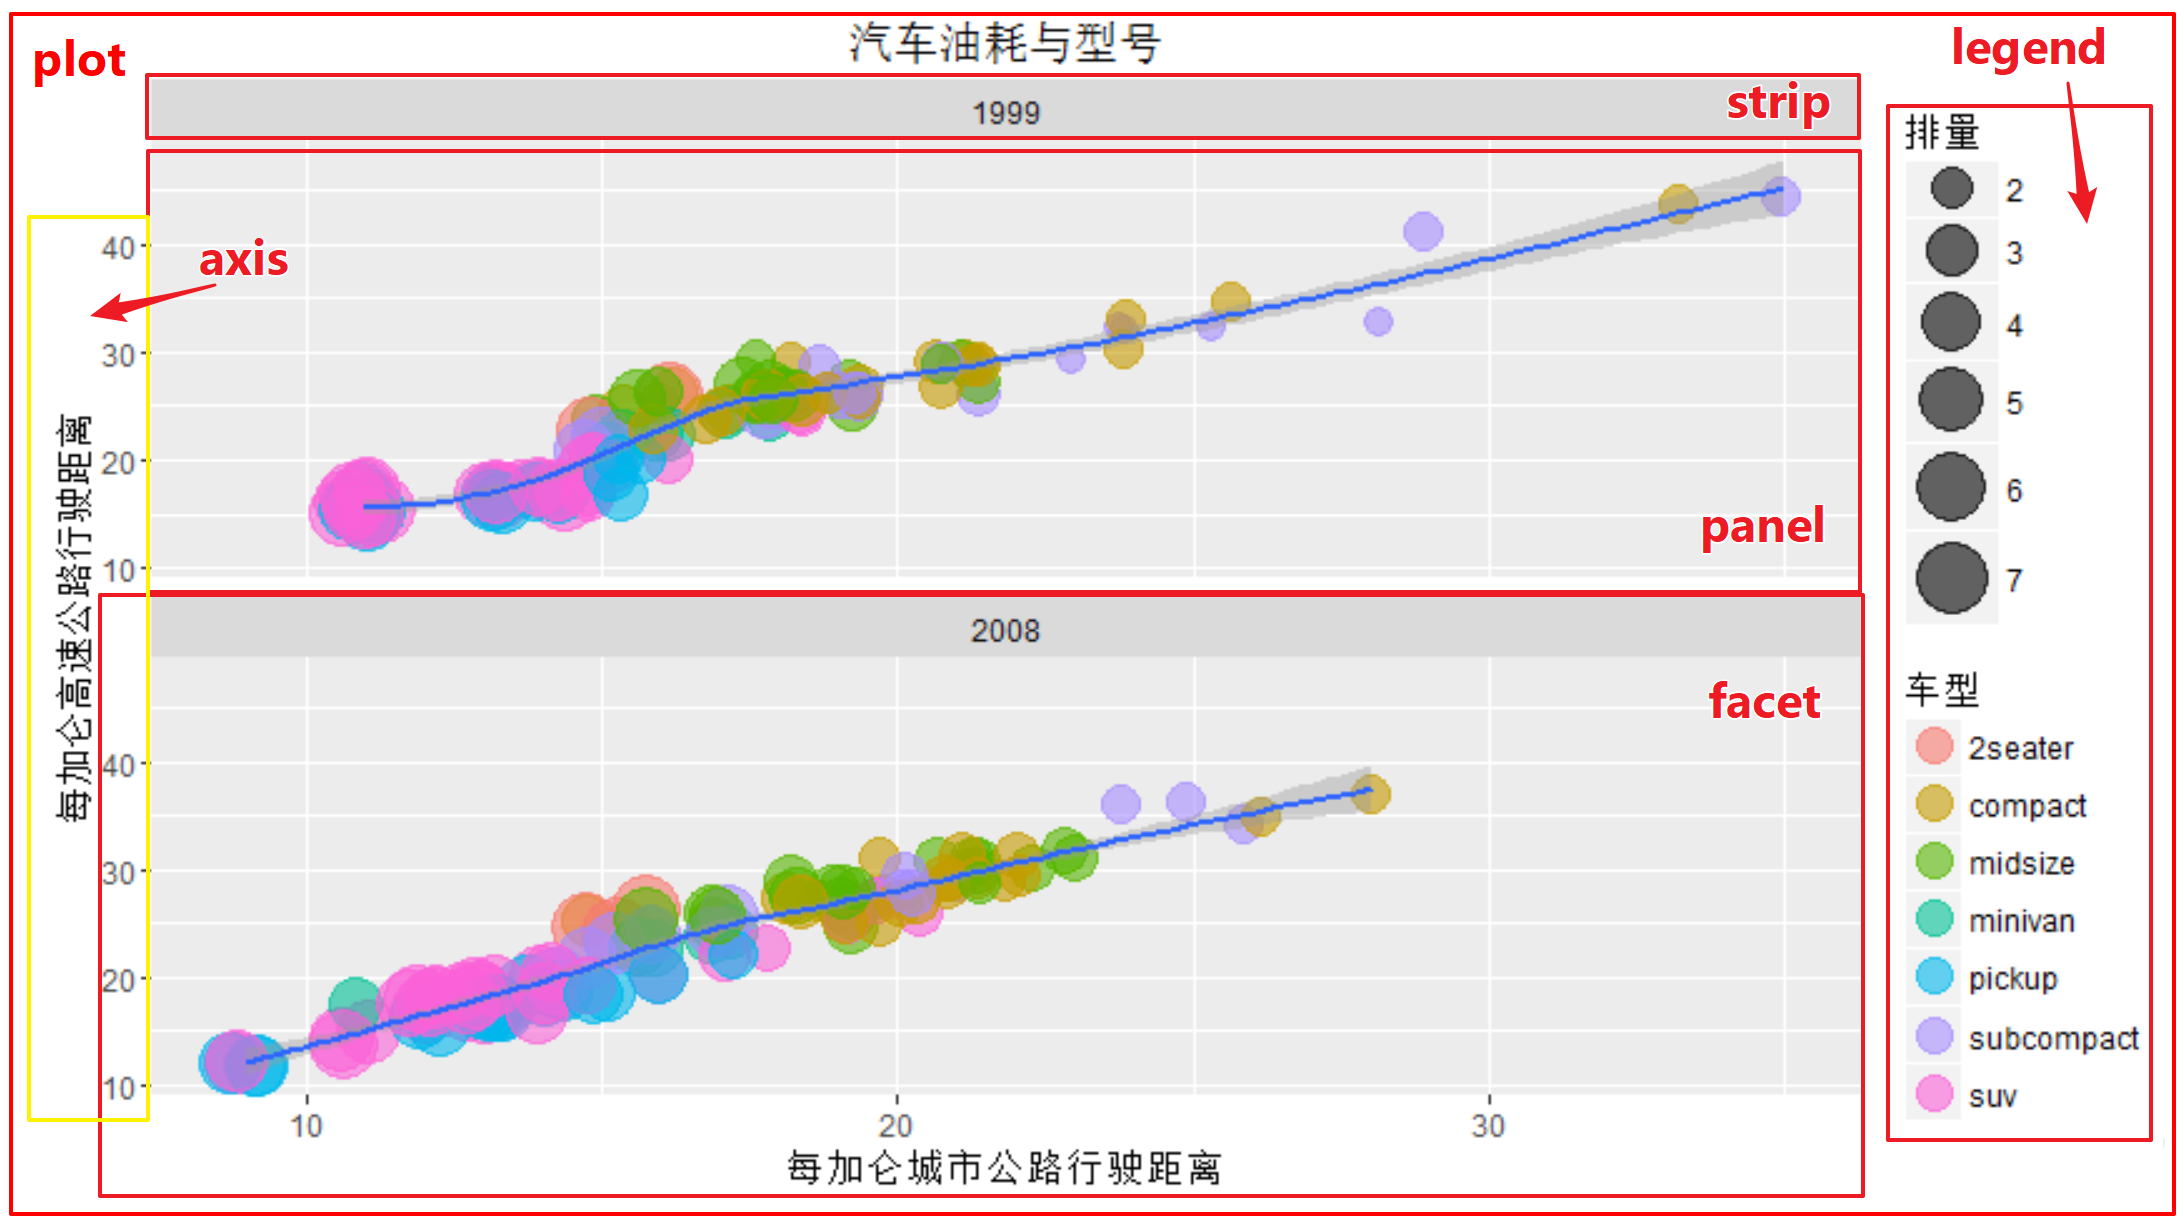
\includegraphics[width=0.9\columnwidth]{ggplot_theme.png}
  \caption{数据无关的图形要素}
\end{figure}}

\only<2>{
\begin{table} \centering \scriptsize
    \renewcommand\arraystretch{0.8}
    \begin{tabular}{>{\centering\arraybackslash} m{0.3\columnwidth} >{\centering\arraybackslash} m{0.1\columnwidth} >{\centering\arraybackslash} m{0.5\columnwidth}}
      \toprule
      \rowcolor{LightCyan}
      \multicolumn{1}{c}{\textbf{要素}} & \multicolumn{1}{c}{\textbf{函数}} &
\multicolumn{1}{c}{\textbf{描述}} \\\hline
      axis.line & element\_line & axis的线 \\
      axis.text.x(y) & element\_text & x,y轴标签\\
      axis.ticks & element\_line & axis刻度线 \\
      axis.title.x(y) & element\_text & axis刻度标签\\
      legend.background & element\_rect & legend背景\\
      legend.key & element\_rect & legend标示背景\\
      legend.text & element\_text & legend标签\\
      legend.title & element\_text & legend标题\\
      panel.background & element\_rect & panel背景\\
      panel.grid.major(minor) & element\_line & panel网格线样式\\
      plot.background & element\_rect & plot背景\\
      plot.title & element\_text & plot标题\\
      strip.background & element\_rect & strip背景\\
      strip.text.x(y) & element\_text & strip文字\\
      \bottomrule
    \end{tabular}
    \caption{theme要素(详见?theme帮助)}
\end{table}}
\end{overlayarea}
\end{frame}

\begin{frame}[t,fragile]{\subsecname}{数据相关的图形要素}
\begin{itemize}
\item 数据相关的图形要素\emphText{负责构造统计数据的绘制图形},大致可以分为数据层、几何图形层和美学层三类
\end{itemize}

\begin{overlayarea}{\textwidth}{\textheight}
\only<1>{
\begin{table} \centering \scriptsize
    \begin{tabular}{|>{\centering\arraybackslash} m{0.3\columnwidth}|>{\centering\arraybackslash} m{0.35\columnwidth}|>{\centering\arraybackslash} m{0.25\columnwidth}|}
      \toprule
      \rowcolor{LightCyan}
      \multicolumn{1}{|c|}{\textbf{语法要素}} & \multicolumn{1}{c|}{\textbf{描述}} &
\multicolumn{1}{c|}{\textbf{对应函数}} \\\hline
      数据(data) & 绘图的数据,必须是data.frame类型 & data.frame() \\\hline
      映射(mapping) & 将数据按变量映射为图形要素 & aes()\\\hline
      几何对象(geometric object) & 用来展示数据的几何对象 & geom\_XXX()、annotate() \\\hline
      统计变换(statistical transformations) & 对原始数据进行统计变换计算 & stat\_XXX()\\\hline
      标度(scales) & 变量映射到图形要素的标度,体现为图例和坐标刻度 & scale\_XXX()、labs()、guides()\\\hline
      坐标系(coordinate system) & 绘图坐标系统 & coord\_XXX()\\\hline
      位置调整(position adjustments) & 对图形元素位置做精细控制 & position\_XXX()\\\hline
      分面(faceting) & 在不同网格中绘制图形,类似lattice & facet\_XXX()\\
      \bottomrule
    \end{tabular}
    %\caption{ggplot2中的语法要素}
\end{table}}
\end{overlayarea}
\end{frame}

\begin{frame}[t,fragile]{\subsecname}{数据(data)}
\begin{itemize}
\item ggplot2对数据的要求是\emphText{必须是data.frame类型}
\item ggplot2从给定的data.frame中提取绘图所需变量\emphText{生成新的数据集},而不是直接在原数据上进行变换
\item ggplot2允许\emphText{用相同代码、不同数据集进行绘图},只需要用\emphText{“\%+\%”}
添加新的数据集代替原数据集
\end{itemize}

\begin{onlyenv}<2>
\begin{rcode}
# 将绘图内容保存在一个绘图对象p中
> p <- ggplot(mtcars, aes(mpg, wt, colour = cyl)) + geom_point()

# 通过变换重新生成一份新的数据集
> mtcars_new <- transform(mtcars, mpg = mpg ^ 2)

# 按照原来的绘图设定对新数据集进行绘制
> p |\colorbox{green}| mtcars_new
\end{rcode}
\end{onlyenv}
\end{frame}

\begin{frame}[t,fragile]{\subsecname}{映射(mapping)}
\begin{itemize}
\item<1-> \emphText{aes()}函数用来将数据变量映射到图形中,使变量成为可以被感知的图形属性
\item<1-> \emphText{最好不要使用指定数据集之外的变量},这不利于将绘图所需数据都封装到一个对象中
\item<3-> 通过\emphText{group}参数将数据按照变量映射到不同分组进行绘图
\end{itemize}

\begin{overlayarea}{\textwidth}{\textheight}
\begin{onlyenv}<1>
\begin{rcode}
> p <- ggplot(mtcars)
> summary(p)
# mtcars数据集中包括wt和hp两个变量
> data: mpg, cyl, disp, hp, drat, wt, qsec, vs, am, gear, carb [32x11]
  faceting: <ggproto object: Class FacetNull, Facet>
# 将wt和hp两个变量分别映射到x坐标和y坐标
> p <- p + aes(x=wt,y=hp)
> summary(p)
> data: mpg, cyl, disp, hp, drat, wt, qsec, vs, am, gear, carb [32x11]
  |\colorbox{green}{mapping:  x = wt, y = hp}|
  faceting: <ggproto object: Class FacetNull, Facet>
\end{rcode}
\end{onlyenv}

\begin{onlyenv}<2>
\begin{minipage}{\textwidth}
\begin{rcode}
# 按照cyl变量将颜色映射到散点 
> ggplot(mtcars,|\colorbox{green}{aes(mpg,wt,colour=cyl)}|) + geom_point()
\end{rcode}
\end{minipage}

\begin{minipage}{\textwidth}
\centering
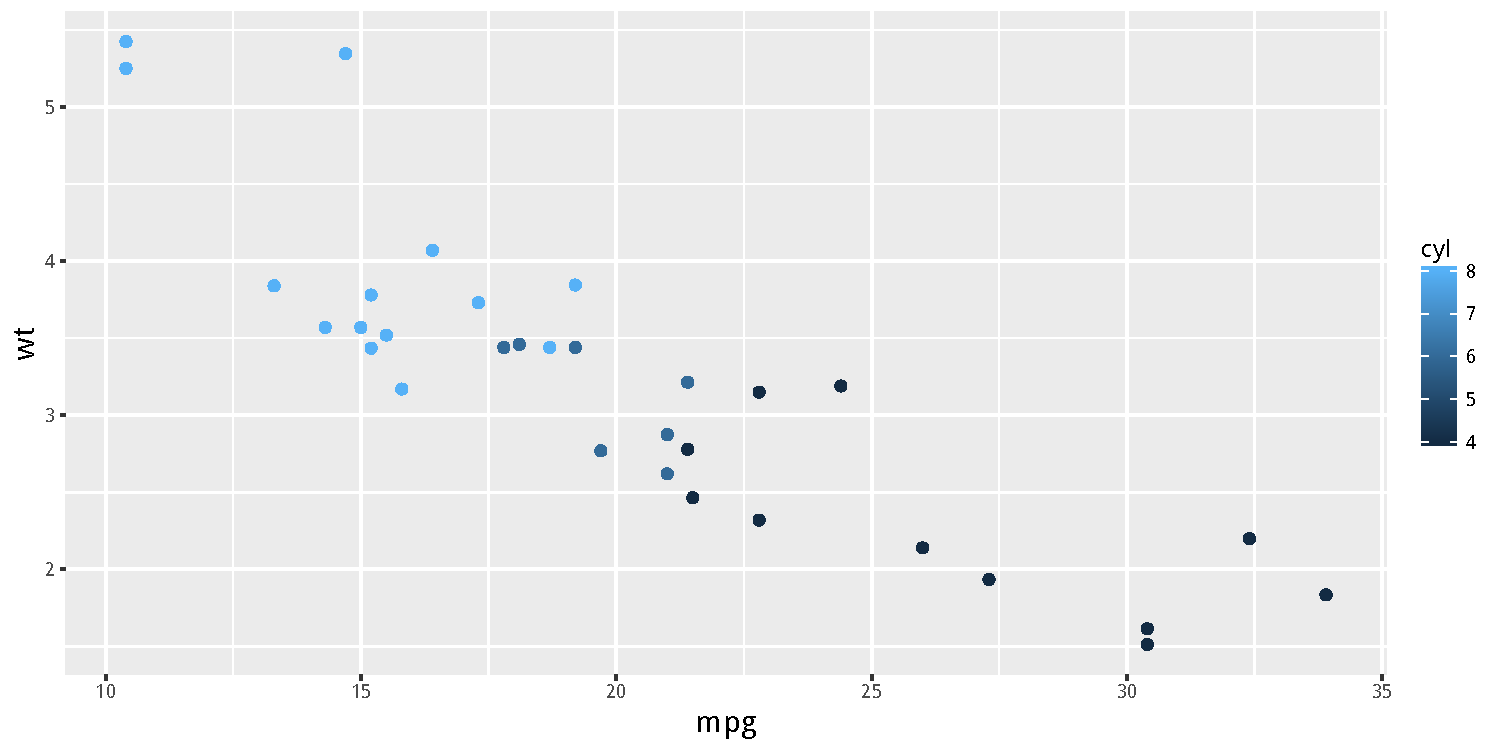
\includegraphics[width=0.9\columnwidth]{ggplot_mapping1.pdf}
\end{minipage}
\end{onlyenv}

\begin{onlyenv}<3>
\begin{minipage}{\textwidth}
\begin{rcode}
# 对Oxboys数据集按照Subject变量分为26个分组
> ggplot(Oxboys, aes(age,height,|\colorbox{green}{group=Subject}|)) + geom_line() +
     geom_smooth(aes(group=1), method = "lm", size = 2, se=F)
\end{rcode}
\end{minipage}

\begin{minipage}{\textwidth}
\centering
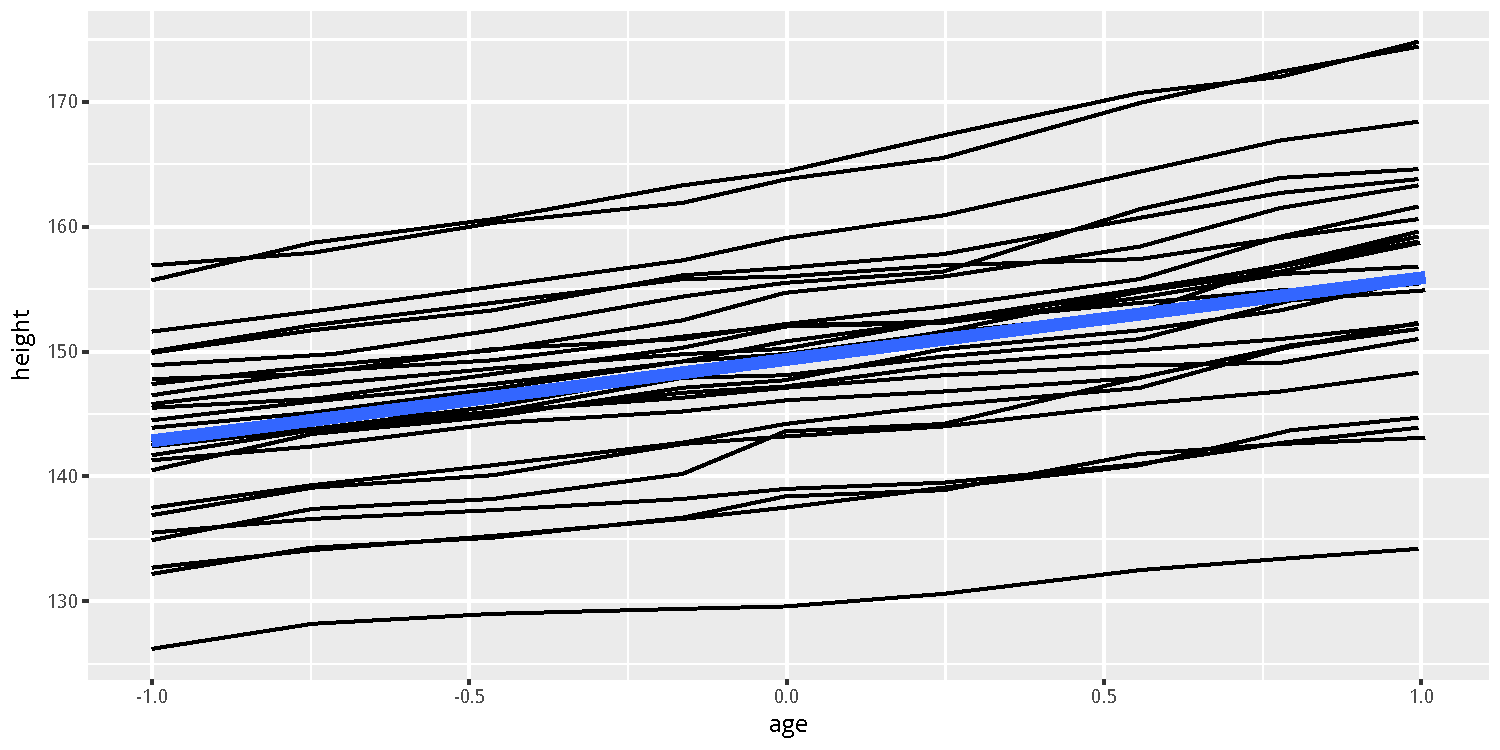
\includegraphics[width=0.9\columnwidth]{ggplot_mapping2.pdf}
\end{minipage}
\end{onlyenv}
\end{overlayarea}
\end{frame}

\begin{frame}[t,fragile]{\subsecname}{标度(scales)}
\begin{itemize}
\item 标度是\emphText{从数据空间的定义域到图形属性空间值域的映射},
将数据转化为视觉上可以感知的颜色、大小、位置和形状
\item ggplot2将标度分为位置标度、颜色标度、手动离散标度和同一型标度,标度函数统一形式为
\emphText{scale\_图形属性\_类型}
\end{itemize}

\begin{overlayarea}{\textwidth}{\textheight}
\only<1>{
\begin{table} \centering \scriptsize
    \renewcommand\arraystretch{0.8}
    \begin{tabular}{>{\centering\arraybackslash} m{0.4\columnwidth} >{\centering\arraybackslash} m{0.2\columnwidth} >{\centering\arraybackslash} m{0.2\columnwidth}}
      \toprule
      \rowcolor{LightCyan}
      \multicolumn{1}{c}{\textbf{图形属性}} & \multicolumn{1}{c}{\textbf{离散型}} & \multicolumn{1}{c}{\textbf{连续型}}\\\hline
      颜色(colour)和填充色(fill) & brewer & \textbf{gradient}\\
      & grey & gradient2 \\
      & \textbf{hue} & gradientn \\
      & identity,manual &\\
      位置(x,y) & \textbf{discrete} & \textbf{continuous}\\
      & & date\\
      形状(shape) & \textbf{shape} & \\
      & identity,manual &\\
      线类型(line type) & \textbf{linetype} & \\
      & identity,manual &\\
      大小(size) & identity,manual & \textbf{size}\\
      \bottomrule
    \end{tabular}
    \caption{按图形属性和变量类型组成的标度函数,默认值为粗体,详见ggplot帮助}
\end{table}}

\begin{onlyenv}<2>
\begin{minipage}{\textwidth}
\begin{rcode}
> p <- qplot(sleep_total, sleep_cycle, data = msleep, colour = vore)
# 通过标度函数scale\_colour\_hue对离散型分类数据集按变量进行颜色值映射
> p + |\colorbox{green}{scale\_colour\_hue}|("What does\nit eat?", breaks = c("herbi", "carni", "omni", NA), labels = c("plants", "meat", "both", "don’t know"))
\end{rcode}
\end{minipage}

\begin{minipage}{\textwidth}
\centering
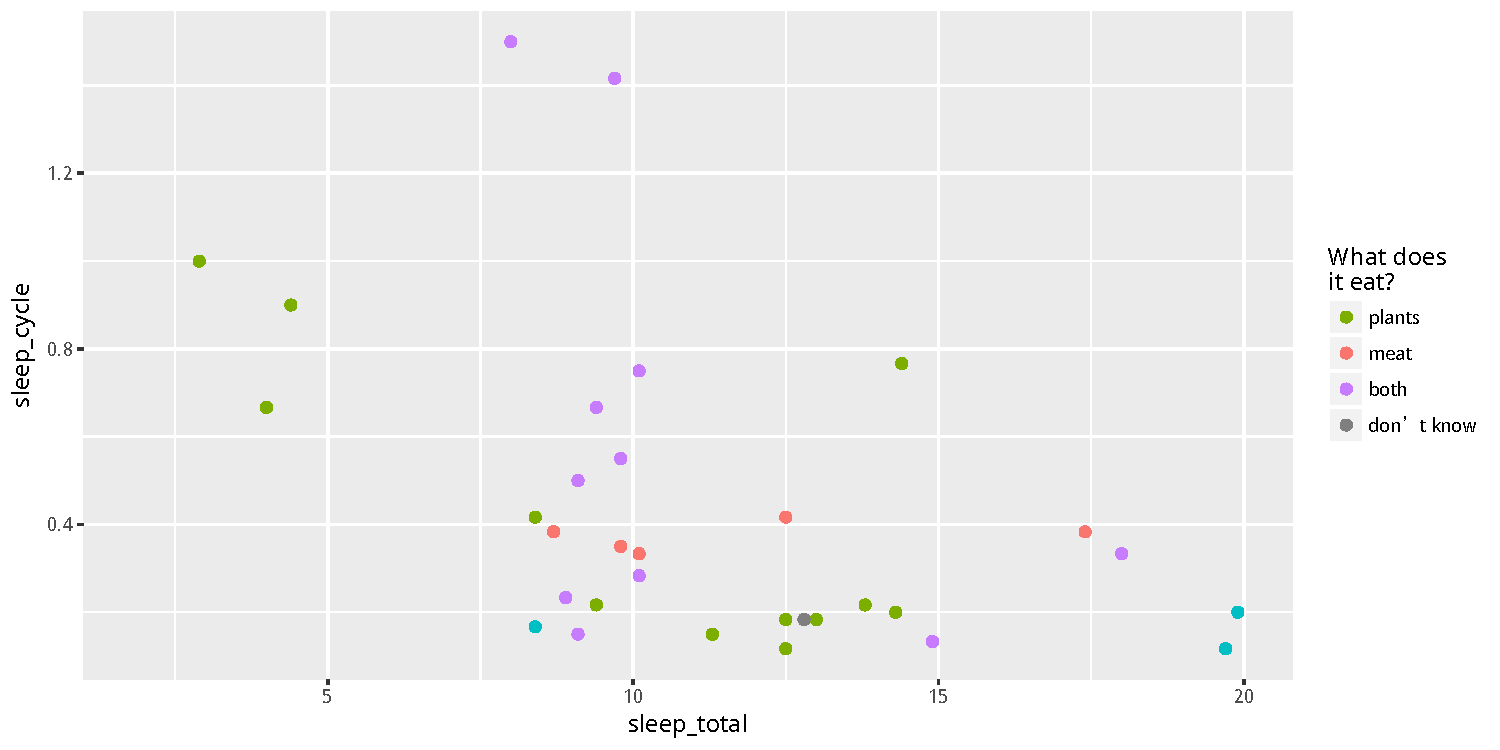
\includegraphics[width=0.9\columnwidth]{ggplot_scales.pdf}
\end{minipage}
\end{onlyenv}
\end{overlayarea}
\end{frame}

\begin{frame}[t,fragile]{\subsecname}{几何对象(geometric object)}
\begin{itemize}
\item 几何对象简称geom,负责执行图形的实际渲染,控制生成的图形类型,
几何对象函数的命名规则是\emphText{geom\_加上几何对象名字}
\end{itemize}
\begin{table} \centering \scriptsize
    \renewcommand\arraystretch{0.8}
    \begin{tabular}{>{\centering\arraybackslash} m{0.3\columnwidth} >{\centering\arraybackslash} m{0.6\columnwidth}}
      \toprule
      \rowcolor{LightCyan}
      \multicolumn{1}{c}{\textbf{函数}} & \multicolumn{1}{c}{\textbf{描述}} \\\hline
      geom\_abline & 由斜率和截距确定的线图\\
      geom\_bar & 条形图\\
      geom\_blank & 空对象,即什么都不绘制\\
      geom\_boxplot & 箱线图\\
      geom\_contour & 等高线图\\
      geom\_density & 核密度图\\
      geom\_histogram & 直方图\\
      geom\_hline & 水平线\\
      geom\_line & 线\\
      geom\_point & 点\\
      geom\_polygon & 多边形\\
      geom\_quantile & 分位数线\\
      geom\_rect & 矩形\\
      geom\_segment & 线段\\
      geom\_smooth & 平滑条件均值图\\
      geom\_text & 文本\\
      \bottomrule
    \end{tabular}
    \caption{部分几何对象快捷函数,详见ggplot帮助}
\end{table}
\end{frame}

\begin{frame}[t,fragile]{\subsecname}{统计变换(statistical transformations)}
\begin{itemize}
\item 统计变换简称stat,负责通过某种方式对数据进行统计汇总,统计变换函数的命名规则是\emphText{stat\_加上统计变换名字}
\end{itemize}
\begin{table} \centering \scriptsize
    \renewcommand\arraystretch{0.9}
    \begin{tabular}{>{\centering\arraybackslash} m{0.3\columnwidth} >{\centering\arraybackslash} m{0.6\columnwidth}}
      \toprule
      \rowcolor{LightCyan}
      \multicolumn{1}{c}{\textbf{函数}} & \multicolumn{1}{c}{\textbf{描述}} \\\hline
      stat\_abline & 添加由斜率和截距确定的线\\
      stat\_bin & 计算封箱数据\\
      stat\_boxplot & 计算组成箱线图的各种元素值\\
      stat\_contour & 绘制三维等高线图\\
      stat\_density & 绘制核密度图\\
      stat\_function & 添加函数曲线\\
      stat\_hline & 添加水平线\\
      stat\_identity & 不做任何变换,添加原始数据\\
      stat\_qq & 计算QQ图的相关值\\
      stat\_quantile & 计算连续分位数\\
      stat\_smooth & 添加平滑曲线\\
      stat\_sum & 计算每个单一值的频数\\
      stat\_summary & 对每个x对应的y值做统计描述\\
      \bottomrule
    \end{tabular}
    \caption{部分统计变换函数,详见ggplot帮助}
\end{table}
\end{frame}

\begin{frame}[t,fragile]{\subsecname}{分面(faceting)}
\begin{itemize}
\item<1-> 分面即在同一图幅上自动摆放多个图形的绘图概念(同lattice)
\item<1-> 提供两种分面类型:\emphText{网格型}(facet\_grid)和\emphText{封装型}(facet\_wrap)
\item<2-> 分面有\emphText{分面变量和控制标度}两个属性;分面变量定义网格的排列,控制标度对分面的坐标进行控制
\end{itemize}

\begin{overlayarea}{\textwidth}{\textheight}
\only<1>{
\begin{figure}[ht]
    \centering
    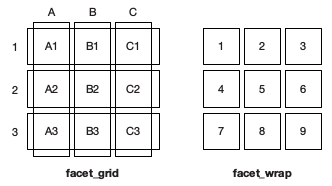
\includegraphics[width=0.7\columnwidth]{ggplot_facet1.png}
    \caption{左图的网格型分面生成一个二维面板网格,面板的行和列通过变量定义;右图的封装型是一个一维面板网格,
按照空间范围封装成二维,这和lattice的网格生成方式是一样的}
\end{figure}}

\only<2>{
\begin{table} \centering \scriptsize
    \renewcommand\arraystretch{1}
    \begin{tabular}{>{\centering\arraybackslash} m{0.1\columnwidth} >{\centering\arraybackslash} m{0.2\columnwidth} >{\centering\arraybackslash} m{0.6\columnwidth}}
      \toprule
      \rowcolor{LightCyan}
      \multicolumn{1}{c}{\textbf{分面变量}} & \multicolumn{1}{c}{\textbf{表达方式}} & \multicolumn{1}{c}{\textbf{描述}}\\\hline
      一行多列 & $.\sim a$ & 按变量a分面,行为1,列为length(a),即横向分面\\
      一列多行 & $a\sim .$ & 按变量a分面,列为1,行为length(a),即纵向分面\\
      多行多列 & $a\sim b$ & 按照变量a和b分面,行为length(a),列为length(b)\\
      额外参数 & space=“free” & 按照图形y轴,或x轴比例,自由分配空间\\
      \bottomrule
    \end{tabular}
    \caption{网格型分面变量属性}
\end{table}
\begin{table} \centering \scriptsize
    \renewcommand\arraystretch{1}
    \begin{tabular}{>{\centering\arraybackslash} m{0.3\columnwidth} >{\centering\arraybackslash} m{0.6\columnwidth}}
      \toprule
      \rowcolor{LightCyan}
      \multicolumn{1}{c}{\textbf{表达方式}} & \multicolumn{1}{c}{\textbf{描述}}\\\hline
       $\sim a+b+c,ncol,nrow$ & 类似lattice,按照变量自定义设置行列网格数\\
      \bottomrule
    \end{tabular}
    \caption{封装型分面变量属性}
\end{table}}

\begin{onlyenv}<3>
\begin{minipage}{\textwidth}
\begin{rcode}
> mpg2 <- subset(mpg, cyl != 5 & drv %in% c("4", "f"))
# 网格型分面变量,行为dry变量,包括4和f两个值;列为cyl变量,包括4,6,8三个值
> ggplot(mpg2, aes(cty,hwy)) + geom_point() + |\colorbox{green}{facet\_grid}|(drv ~ cyl)
\end{rcode}
\end{minipage}
\begin{minipage}{\textwidth}
\begin{figure}
\centering
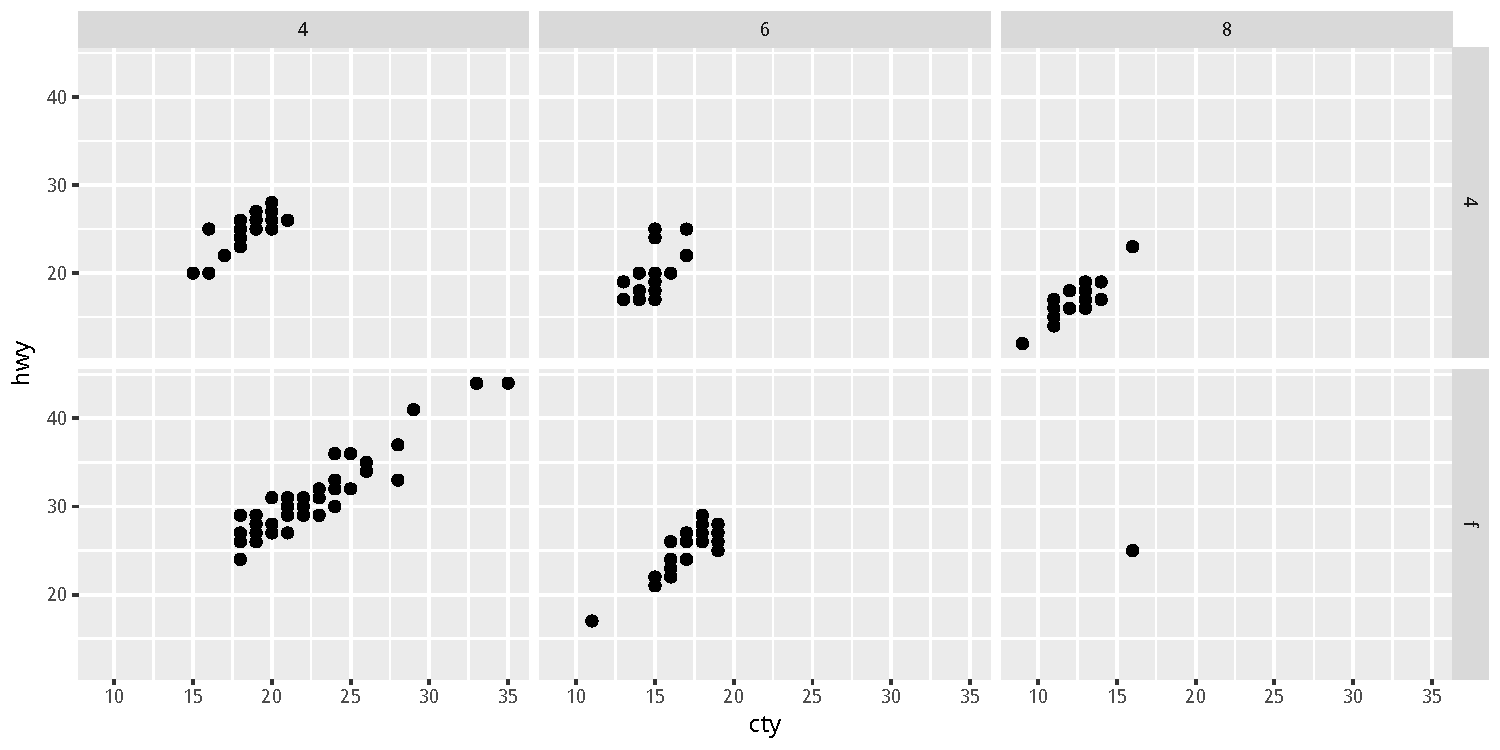
\includegraphics[width=0.85\columnwidth]{ggplot_facet2.pdf}
\caption{网格型分面变量的示例}
\end{figure}
\end{minipage}
\end{onlyenv}

\begin{onlyenv}<4>
\begin{minipage}{\textwidth}
\begin{rcode}
> movies$decade <- round_any(movies$year, 10, floor)
# 封装型分面变量,网格按照decade变量的11个值从左到右排列,如果到达页面边缘则自动从下一行开始排列
> ggplot(subset(movies, decade>1890),aes(rating))+geom_histogram(aes(y=..density..),binwidth=0.5)+ 
     |\colorbox{green}{facet\_wrap}|(~ decade, ncol = 6)
\end{rcode}
\end{minipage}
\begin{minipage}{\textwidth}
\begin{figure}
\centering
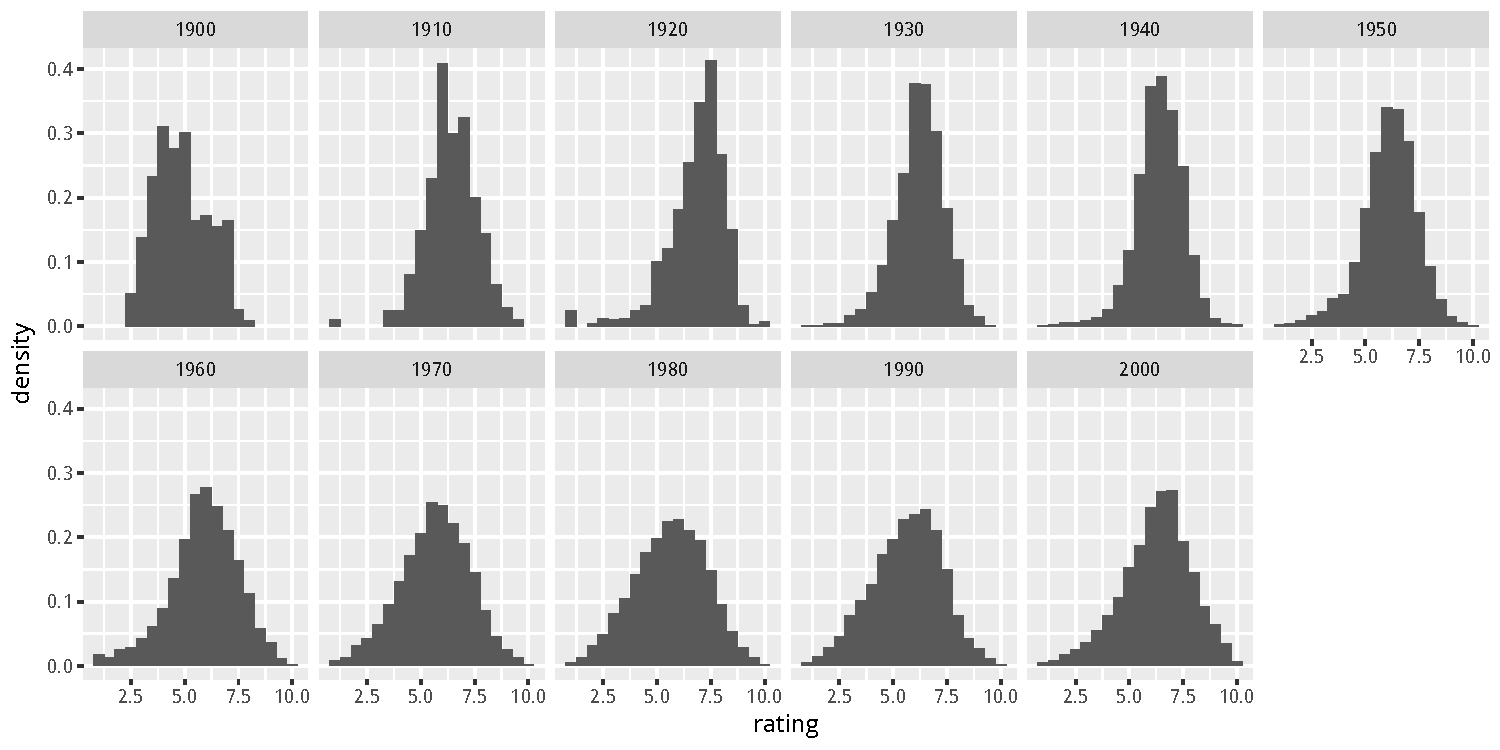
\includegraphics[width=0.8\columnwidth]{ggplot_facet3.pdf}
\caption{封装型分面变量的示例}
\end{figure}
\end{minipage}
\end{onlyenv}

\only<5>{
\begin{table} \centering \scriptsize
    \renewcommand\arraystretch{1}
    \begin{tabular}{>{\centering\arraybackslash} m{0.3\columnwidth} >{\centering\arraybackslash} m{0.6\columnwidth}}
      \toprule
      \rowcolor{LightCyan}
      \multicolumn{1}{c}{\textbf{参数}} & \multicolumn{1}{c}{\textbf{描述}}\\\hline
       \textbf{scales=“fixed”} & x和y的标度在所有分面中都相同\\
       scales=“free” & x和y的标度在每个分面中都可变\\
       scales=“free\_x” & 固定y标度,x标度可变\\
       scales=“free\_y” & 固定x标度,y标度可变\\
      \bottomrule
    \end{tabular}
    \caption{控制标度属性,fixed为默认值}
\end{table}}

\only<6>{\vspace{-15pt}
\begin{figure}[ht]
  \begin{columns}
    \begin{column}{.5\textwidth}\centering
       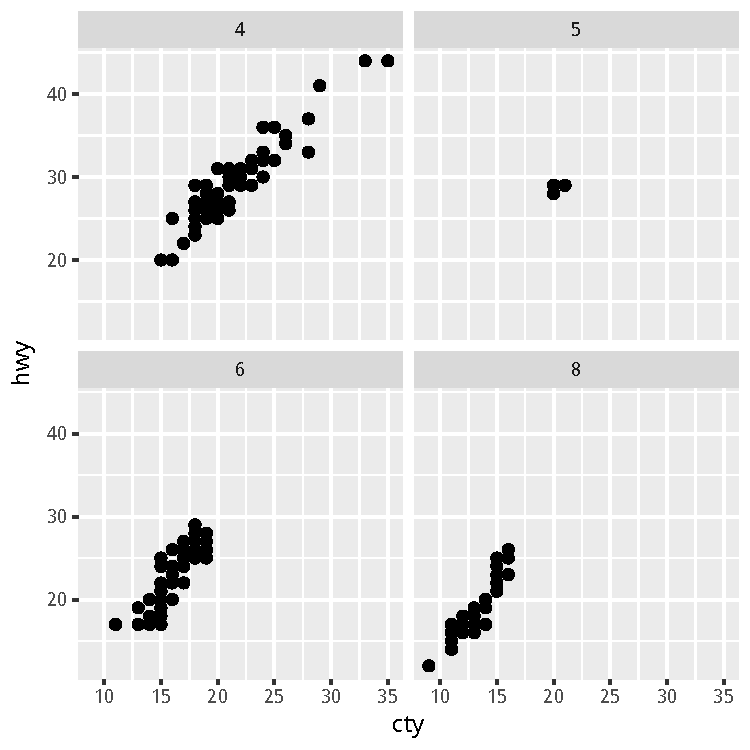
\includegraphics[width=\columnwidth]{ggplot_facet4_1.pdf}
    \end{column}

    \begin{column}[c]{.5\textwidth}\centering
       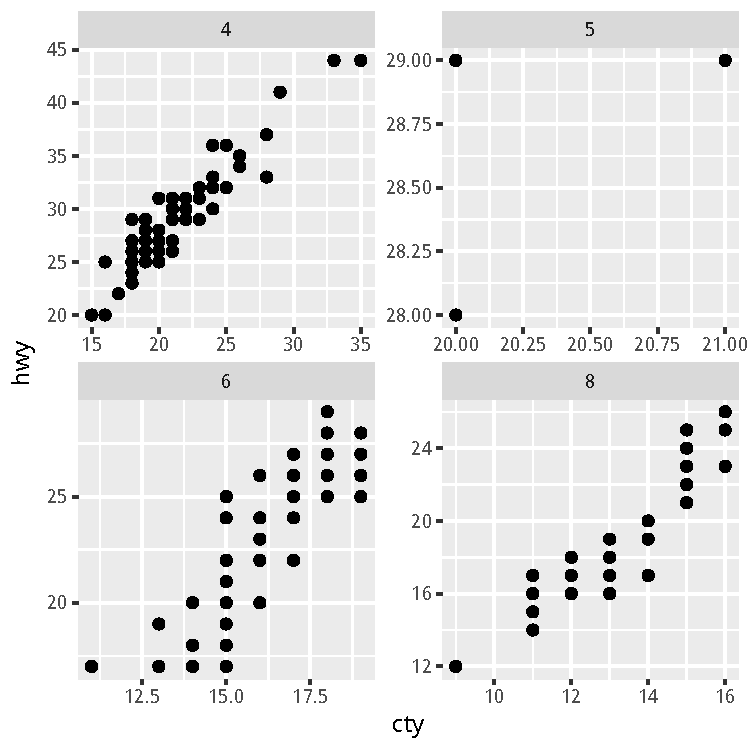
\includegraphics[width=\columnwidth]{ggplot_facet4_2.pdf}
    \end{column}
  \end{columns}
\caption{控制标度的示例.左边是scales=``fixed'',右边是scales=``free''}
\end{figure}}

    % \begin{figure}
    %   \captionsetup[subfigure]{labelformat=empty} 
    %   \subfloat[]
    %   {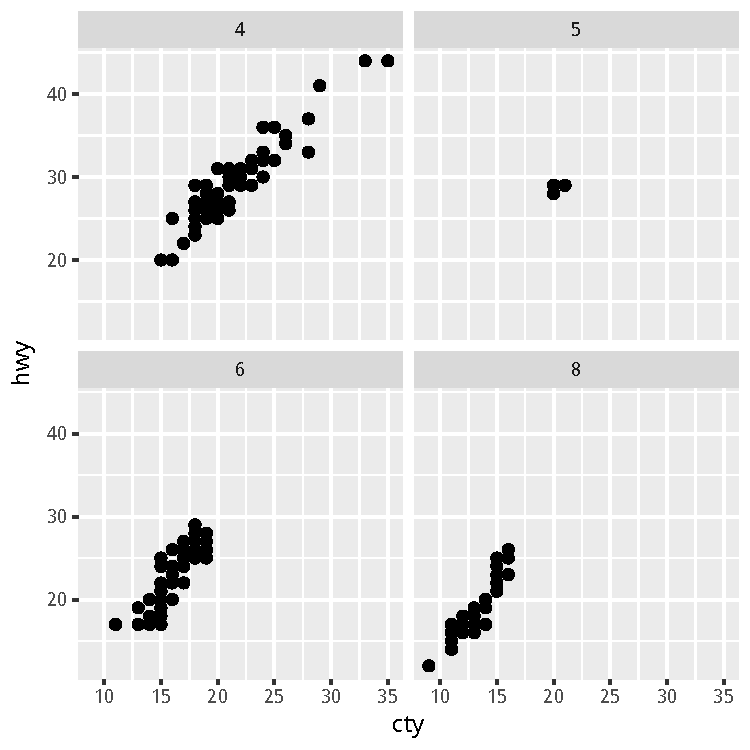
\includegraphics[width=0.48\columnwidth]{ggplot_facet4_1.pdf}} \hspace{1pt}
    %   \subfloat[]
    %   {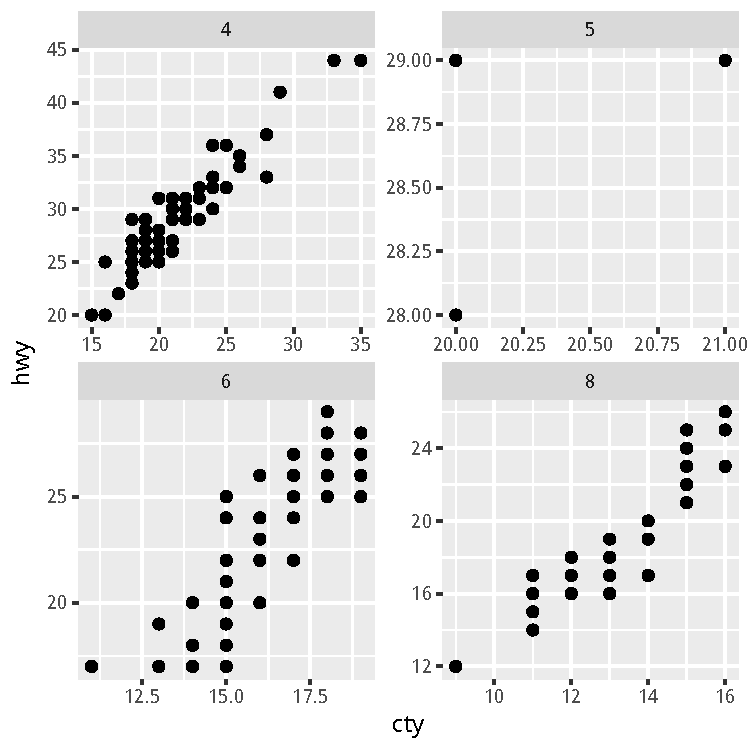
\includegraphics[width=0.48\columnwidth]{ggplot_facet4_2.pdf}}
    %   \caption{控制标度的示例.左边是scales=``fixed'',右边是scales=``free''}
    % \end{figure}\vspace{25pt}}
\end{overlayarea}
\end{frame}

\begin{frame}[t]{\subsecname}{位置调整(position adjustments)}
\begin{itemize}
\item 位置调整指的是对图层中\emphText{元素的位置}进行调整
\item 位置调整\emphText{通常用于离散型数据},通过对位置的微调来比较数据
\end{itemize}

\begin{overlayarea}{\textwidth}{\textheight}
\only<1>{\vspace{15pt}
\begin{table} \centering \scriptsize
    \renewcommand\arraystretch{1}
    \begin{tabular}{>{\centering\arraybackslash} m{0.3\columnwidth} >{\centering\arraybackslash} m{0.5\columnwidth}}
      \toprule
      \rowcolor{LightCyan}
      \multicolumn{1}{c}{\textbf{参数名称}} & \multicolumn{1}{c}{\textbf{描述}} \\\hline
      dodge & 避免重叠,并排放置\\
      fill & 堆叠图形元素并将高度标准化为1\\
      identity & 不做任何调整\\
      jitter & 给点要素添加扰动避免重合\\
      stack & 将图形堆叠起来\\
      \bottomrule
    \end{tabular}
    \caption{ggplot2中提供的5种位置调整参数}
\end{table}}

\only<2>{
    \vspace{15pt}
    \begin{figure} \centering
      \captionsetup[subfigure]{labelformat=empty} 
      \subfloat[position="stack'']
      {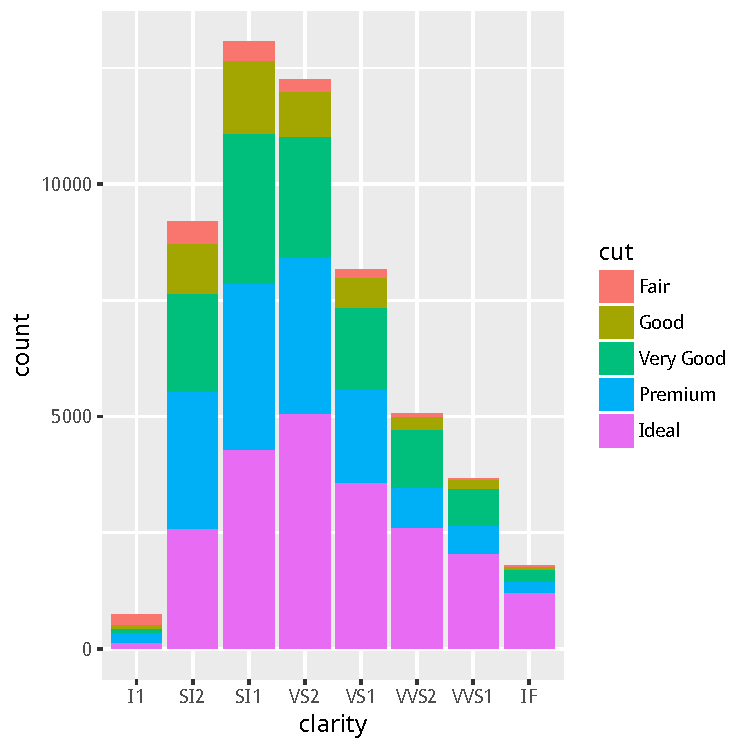
\includegraphics[width=0.3\columnwidth]{ggplot_position1_1.pdf}} \hspace{1pt}
      \subfloat[position="fill'']
      {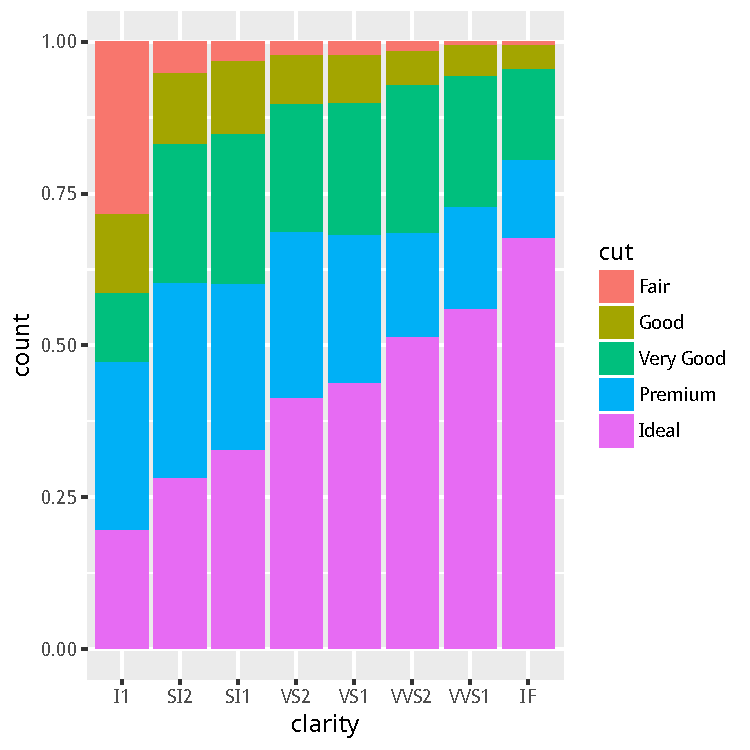
\includegraphics[width=0.3\columnwidth]{ggplot_position1_2.pdf}} \hspace{1pt}
      \subfloat[position="dodge'']
      {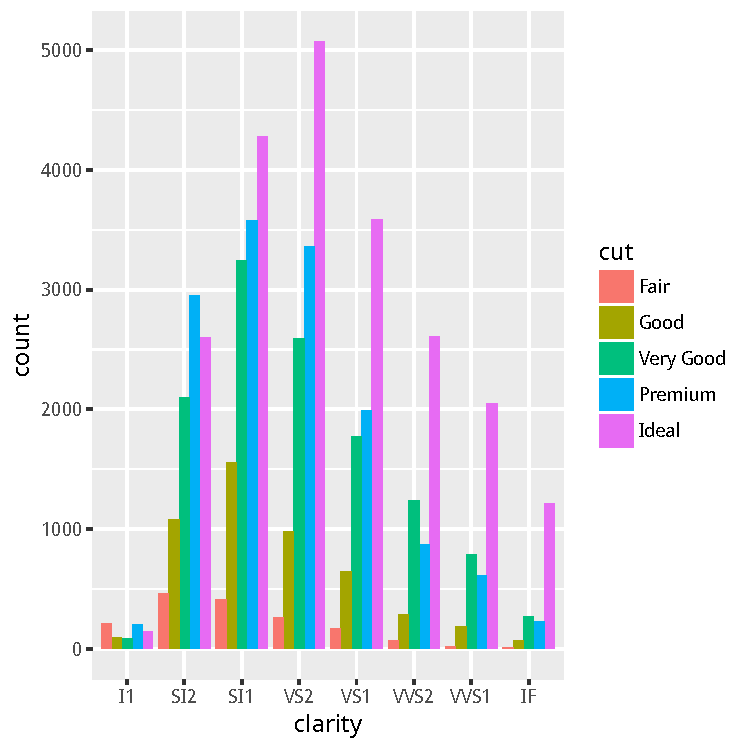
\includegraphics[width=0.3\columnwidth]{ggplot_position1_3.pdf}} 
      \caption{位置调整参数在条形图中应用的示例}
    \end{figure}\vspace{-15pt}}
\end{overlayarea}
\end{frame}

\begin{frame}[t,fragile]{\subsecname}{坐标系(coordinate system)}
\begin{itemize}
\item 坐标系是将两种位置标度结合在一起组成的二维定位系统,坐标系函数命名规则是\emphText{coord\_加上坐标系名字}
\item \emphText{ggplot2包仅支持二维坐标系},要实现三维绘图必须依赖其他第三方包,例如plotly和rgl
\end{itemize}

\begin{overlayarea}{\textwidth}{\textheight}
\only<1>{
\begin{table} \centering \scriptsize
    \renewcommand\arraystretch{1}
    \begin{tabular}{>{\centering\arraybackslash} m{0.3\columnwidth} >{\centering\arraybackslash} m{0.5\columnwidth}}
      \toprule
      \rowcolor{LightCyan}
      \multicolumn{1}{c}{\textbf{坐标系名字}} & \multicolumn{1}{c}{\textbf{描述}} \\\hline
      cartesian & 笛卡尔坐标系\\
      equal & 同尺度笛卡尔坐标系\\
      flip & 翻转的笛卡尔坐标系\\
      trans & 变换的笛卡尔坐标系\\
      map & 地图投影\\
      polar & 极坐标系\\
      \bottomrule
    \end{tabular}
    \caption{ggplot2中可用的坐标系}
\end{table}}

\only<2>{
    \begin{figure} \centering
      \captionsetup[subfigure]{labelformat=empty,textfont=scriptsize} 
      \subfloat[cartesian()]
      {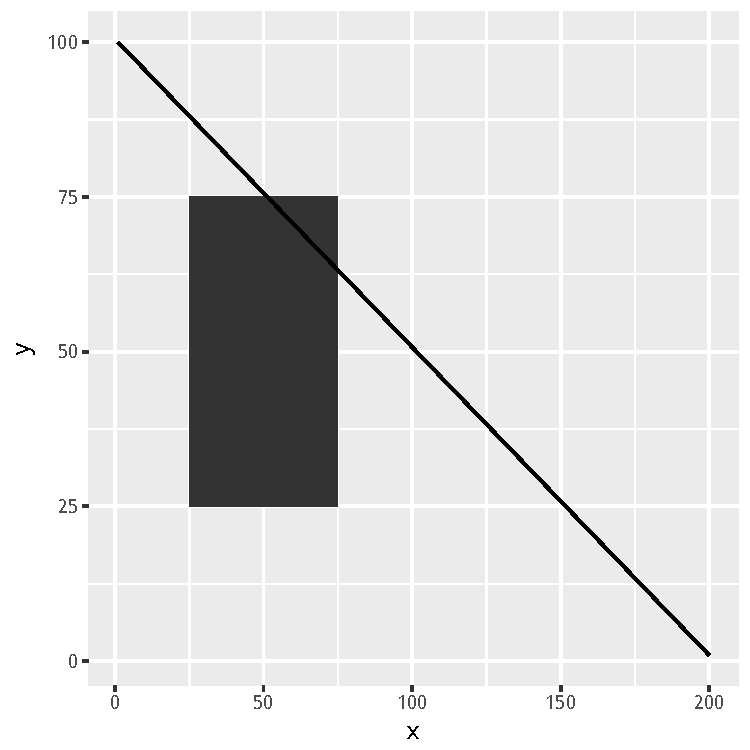
\includegraphics[width=0.2\columnwidth]{ggplot_coord1_1.pdf}} \hspace{20pt}
      \subfloat[polar("x'')]
      {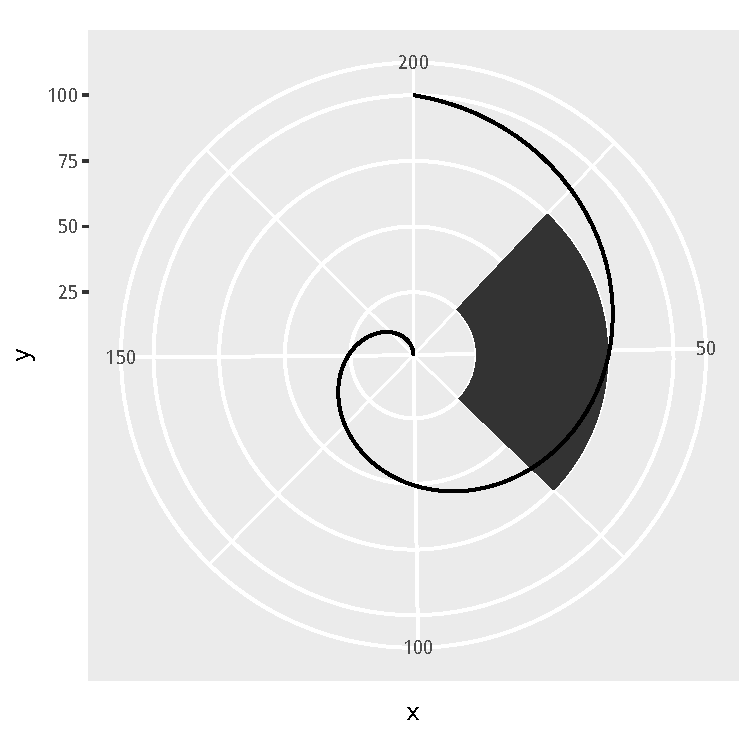
\includegraphics[width=0.2\columnwidth]{ggplot_coord1_2.pdf}} \hspace{20pt}
      \subfloat[polar("y'')]
      {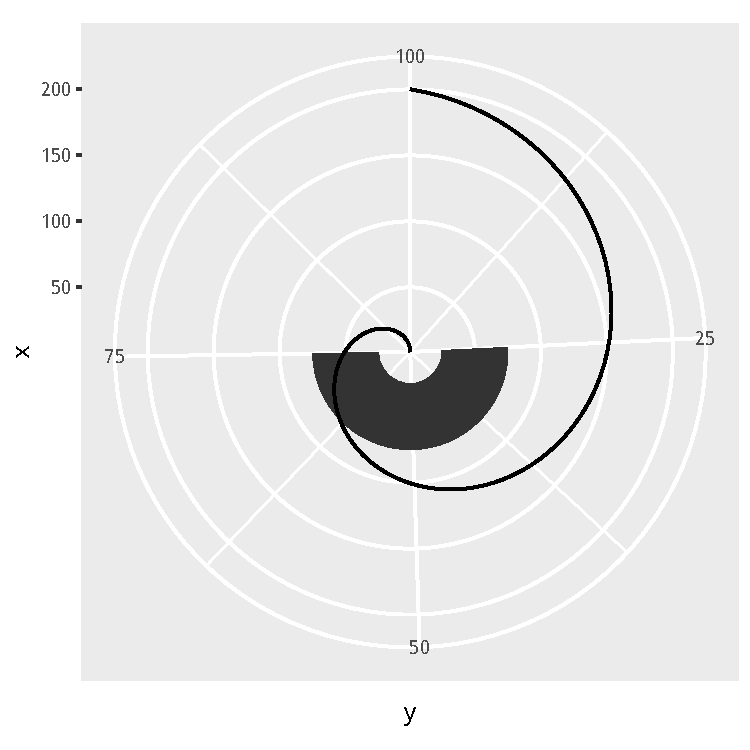
\includegraphics[width=0.2\columnwidth]{ggplot_coord1_3.pdf}} \hspace{20pt}
      \subfloat[flip()]
      {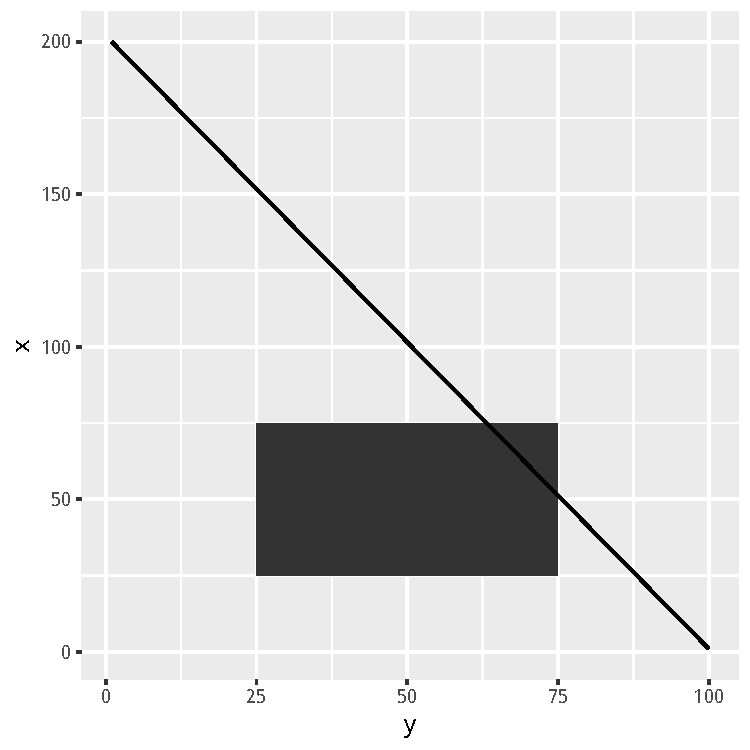
\includegraphics[width=0.2\columnwidth]{ggplot_coord1_4.pdf}} \hspace{20pt}
      \subfloat[trans(y="log10'')]
      {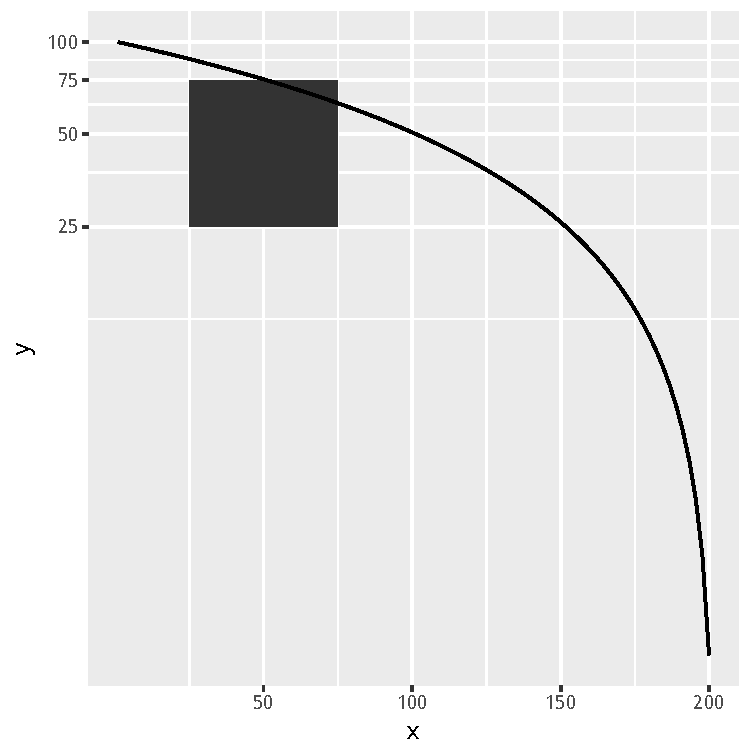
\includegraphics[width=0.2\columnwidth]{ggplot_coord1_5.pdf}} \hspace{20pt}
      \subfloat[equal()]
      {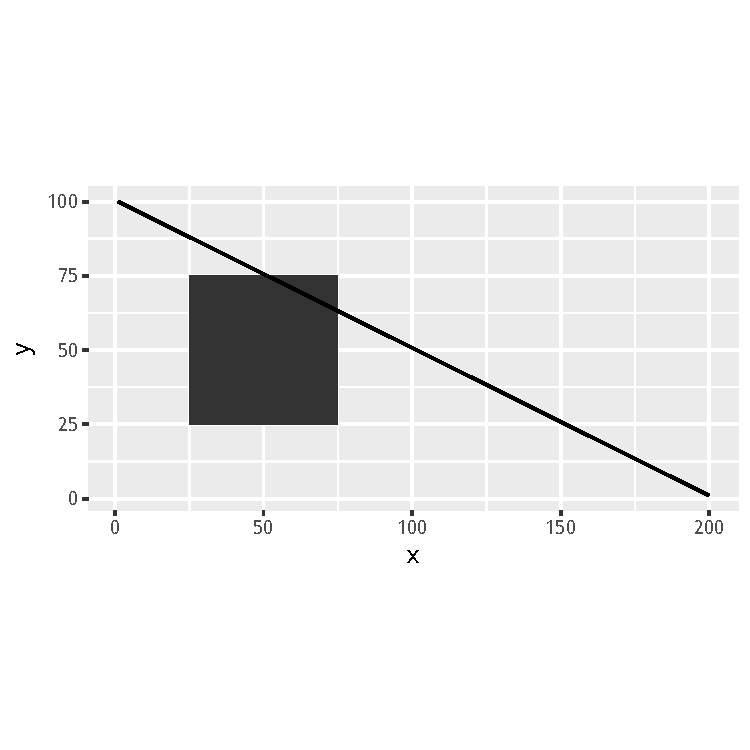
\includegraphics[width=0.2\columnwidth]{ggplot_coord1_6.pdf}} 
      \caption{直线与矩形在不同坐标系的变换示例}
    \end{figure}}
\end{overlayarea}
\end{frame}

%%% https://www.plob.org/article/7665.html
\begin{frame}[t,fragile]{\subsecname}{图层}
\begin{itemize}
\item<1-> 图层是ggplot2特有的概念,其作用是生成在图像上能够被人感知的\emphText{对象}
\item<1-> 图层由五个语法要素组成:数据、映射、统计变换、几何对象和位置调整,可以用\emphText{layer函数}定义
\item<2-> ggplot2的\emphText{快捷函数}(stat\_和geom\_开头)也可以定义图层,简化layer函数的复杂性;
任何图层\emphText{必须包括geom和stat两部分}
\end{itemize}

\begin{overlayarea}{\textwidth}{\textheight}
\begin{onlyenv}<1-2>
\begin{rcode}
# layer函数定义, 其中data和mapping可以从ggplot函数定义的默认值中继承
layer(geom = NULL, stat = NULL, data = NULL, mapping = NULL,
  position = NULL, params = list(), inherit.aes = TRUE,
  check.aes = TRUE, check.param = TRUE, subset = NULL, show.legend = NA)

# ggplot定义数据集(data)和图形属性映射(mapping)
> p <- ggplot(diamonds,aes(x=carat))
# 添加一个自定义图层,并指定相应参数,其中数据集和图形属性映射继承默认值
> p <- p + |\colorbox{green}{layer}|(geom = "bar",stat = "bin",position = "identity"
    params = list(fill = "steelblue", binwidth=0.5))
\end{rcode}
\end{onlyenv}

\begin{onlyenv}<2>
\begin{rcode}
# 任何ggpplot2图层必须包含stat和geom两部分
geom_XXX(data, mapping, ..., stat, position)
stat_XXX(data, mapping, ..., geom, position)

# 以下两条绘图语句得到的结果是完全一样的
ggplot(diamonds,aes(x=carat)) + |\colorbox{green}{geom\_histogram}|(fill="steelblue",|\colorbox{green}{stat}|="bin", binwidth=0.5)
ggplot(diamonds,aes(x=carat)) + |\colorbox{green}{stat\_bin}|(fill="steelblue",|\colorbox{green}{geom}|="bar", binwidth=0.5)
\end{rcode} 
\end{onlyenv}
\end{overlayarea}
\end{frame}

\begin{frame}{\subsecname}{绘图过程}
\begin{figure}[ht]
  \begin{columns}
    \begin{column}{.6\textwidth}\centering
  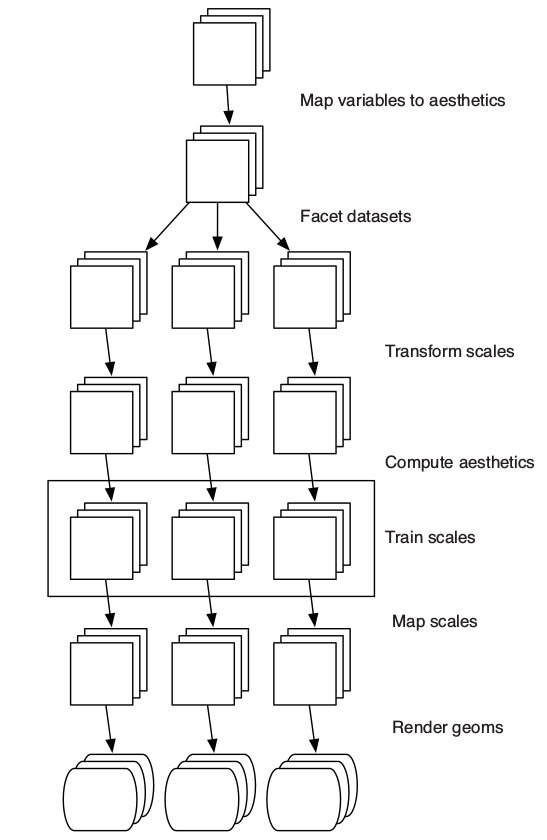
\includegraphics[width=0.75\columnwidth]{ggplot_flow.png}
    \end{column}

    \begin{column}[c]{.4\textwidth}
  \caption{ggplot2中处理图形绘制的全过程,本图中每个方框表示一个图层,包含三个图层和三个分面.除了train scales之外,其他步骤都对每个小数据集做变换.}
    \end{column}
  \end{columns}
\end{figure}
\end{frame}

\begin{frame}[c,fragile]{\subsecname}{绘图过程}

\begin{onlyenv}<1>
\begin{minipage}{\textwidth}
\begin{rcode}
# 第一步:初始化,载入数据并进行图形属性映射
> ggplot(mpg, aes(x=cty, y=hwy))
\end{rcode}
\end{minipage}
\begin{minipage}{\textwidth}
\centering
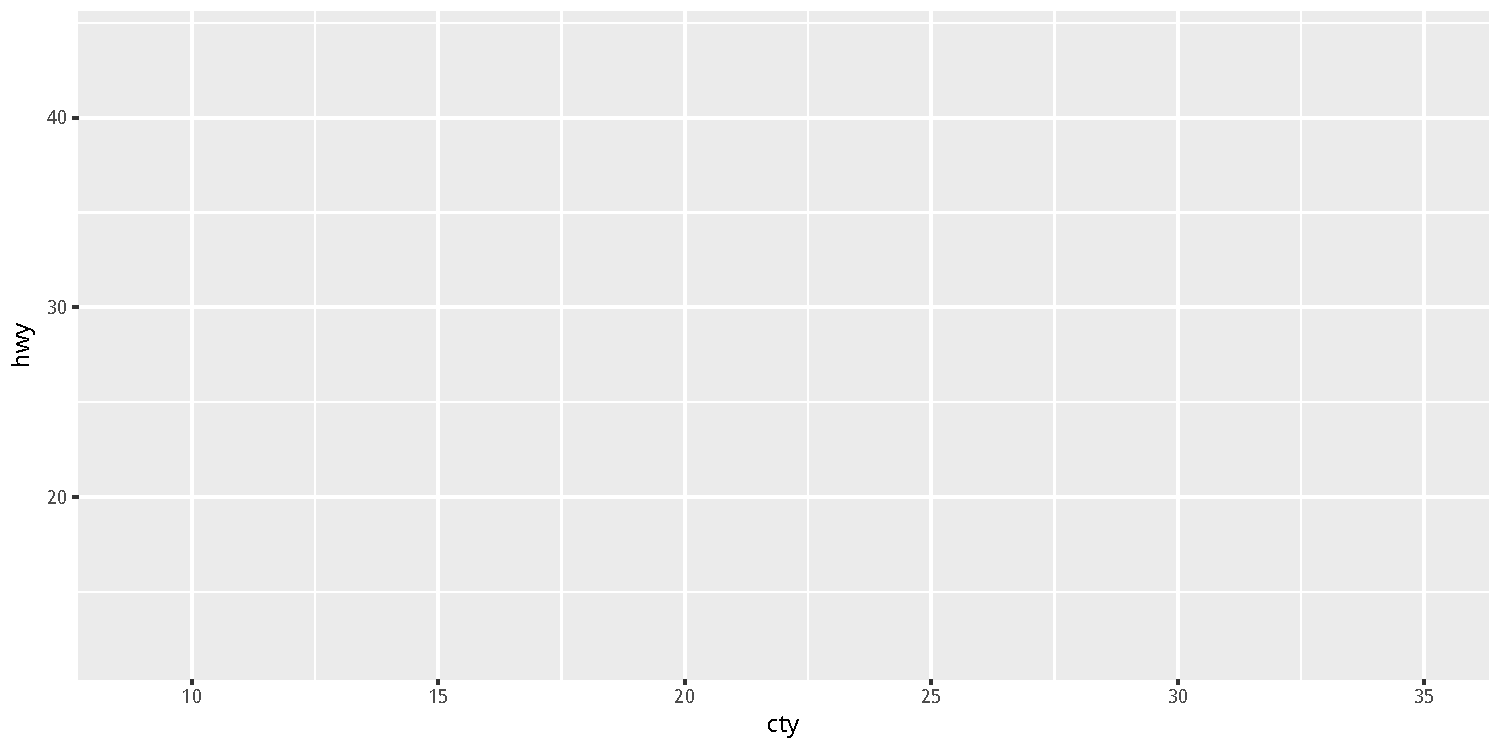
\includegraphics[width=\columnwidth]{ggplot_example1.pdf}
\end{minipage}
\end{onlyenv}

\begin{onlyenv}<2>
\begin{minipage}{\textwidth}
\begin{rcode}
# 第二步:分面,按年份
> ggplot(mpg, aes(x=cty, y=hwy))+
      facet_wrap(~ year,ncol=2)
\end{rcode}
\end{minipage}
\begin{minipage}{\textwidth}
\centering
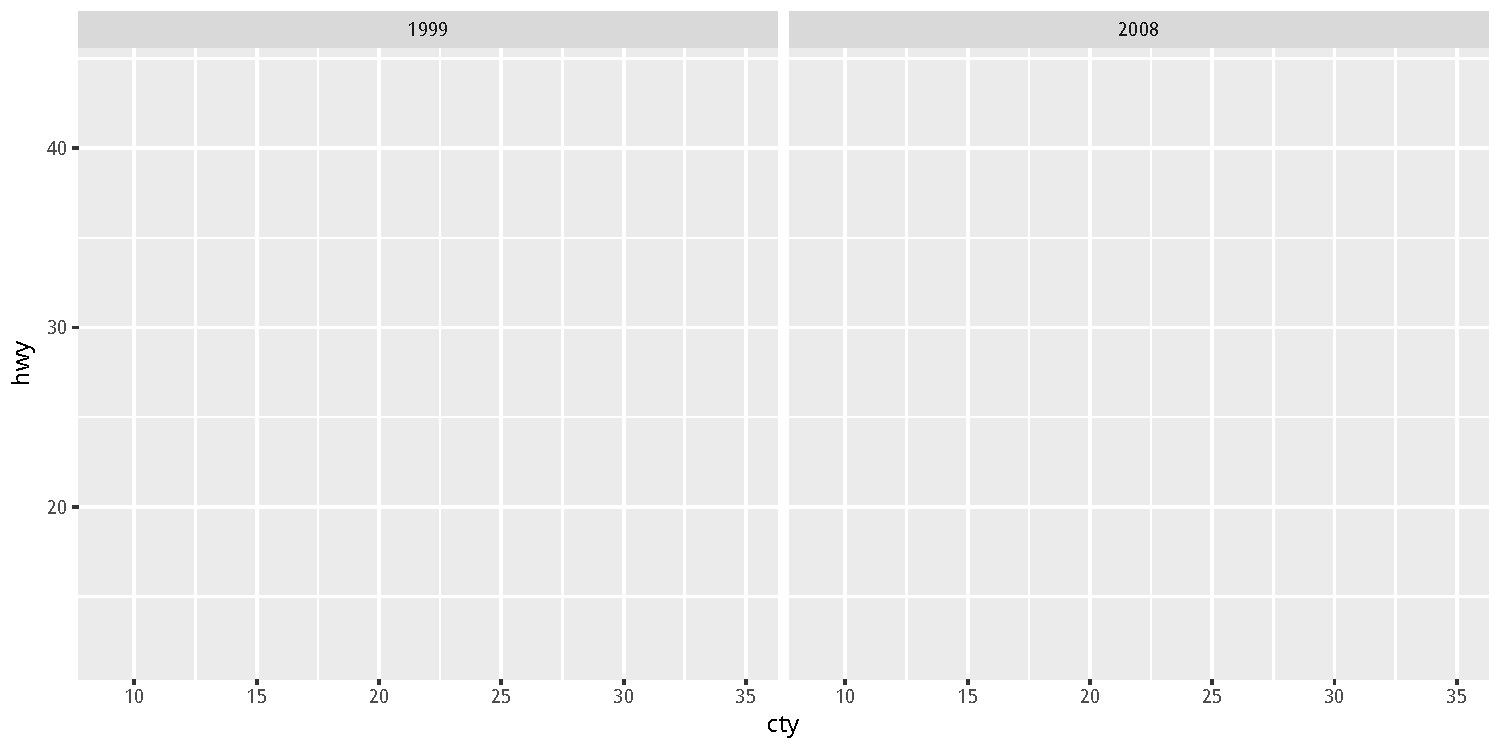
\includegraphics[width=\columnwidth]{ggplot_example2.pdf}
\end{minipage}
\end{onlyenv}

\begin{onlyenv}<3>
\begin{minipage}{\textwidth}
\begin{rcode}
# 第三步:绘制图层,包括几何对象图层、经过统计变换后的图层和位置调整
> ggplot(mpg, aes(x=cty, y=hwy))+
      facet_wrap(~ year,ncol=2)+
      geom_point(aes(colour=class,size=displ),alpha=0.6,position = "jitter")+  
      stat_smooth()
\end{rcode}
\end{minipage}
\begin{minipage}{\textwidth}
\centering
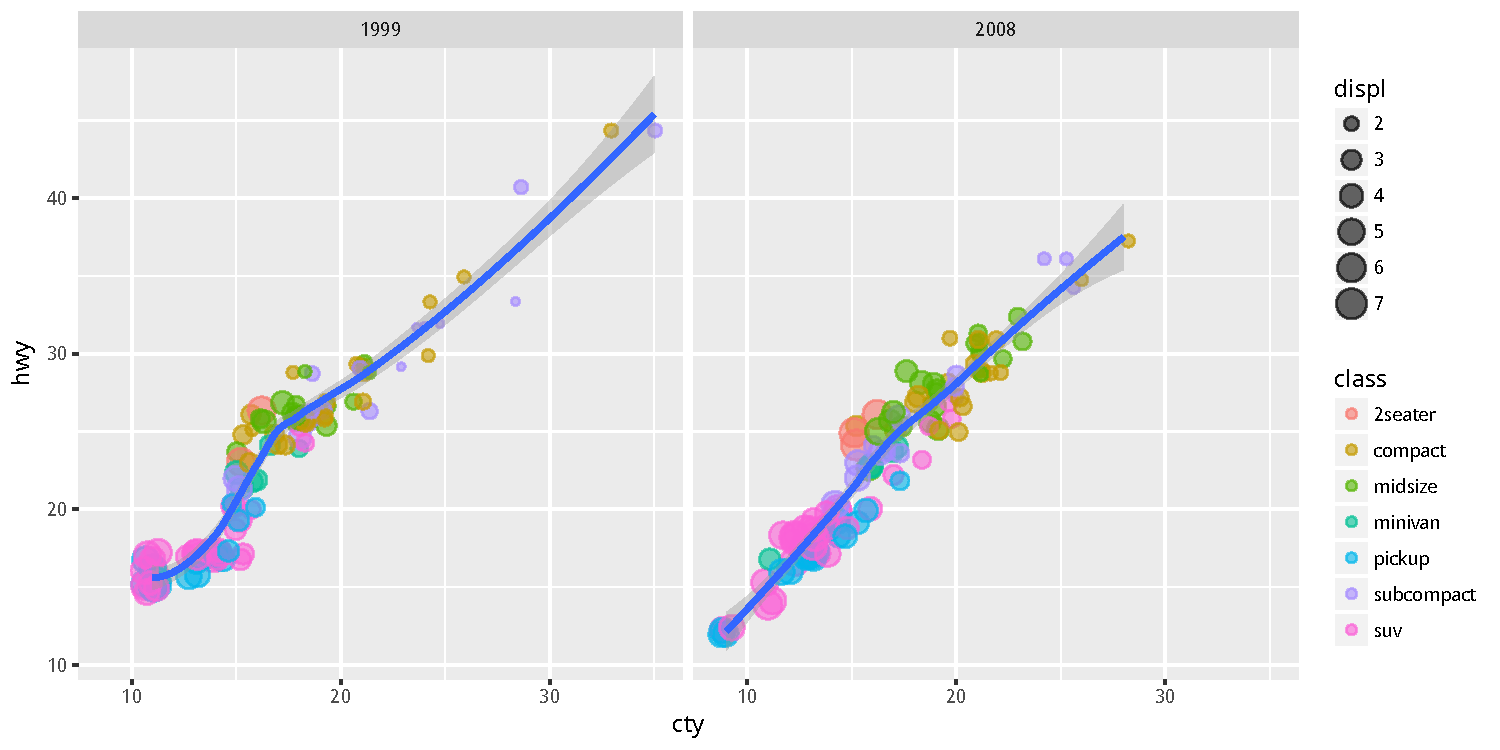
\includegraphics[width=\columnwidth]{ggplot_example3.pdf}
\end{minipage}
\end{onlyenv}

\begin{onlyenv}<4>
\begin{minipage}{\textwidth}
\begin{rcode}
# 第四步:训练标度,表现为散点的大小
> ggplot(mpg, aes(x=cty, y=hwy))+
      facet_wrap(~ year,ncol=2)+
      geom_point(aes(colour=class,size=displ),alpha=0.6,position = "jitter")+  
      stat_smooth()+  
      scale_size(range = c(5, 10))
\end{rcode}
\end{minipage}
\begin{minipage}{\textwidth}
\centering
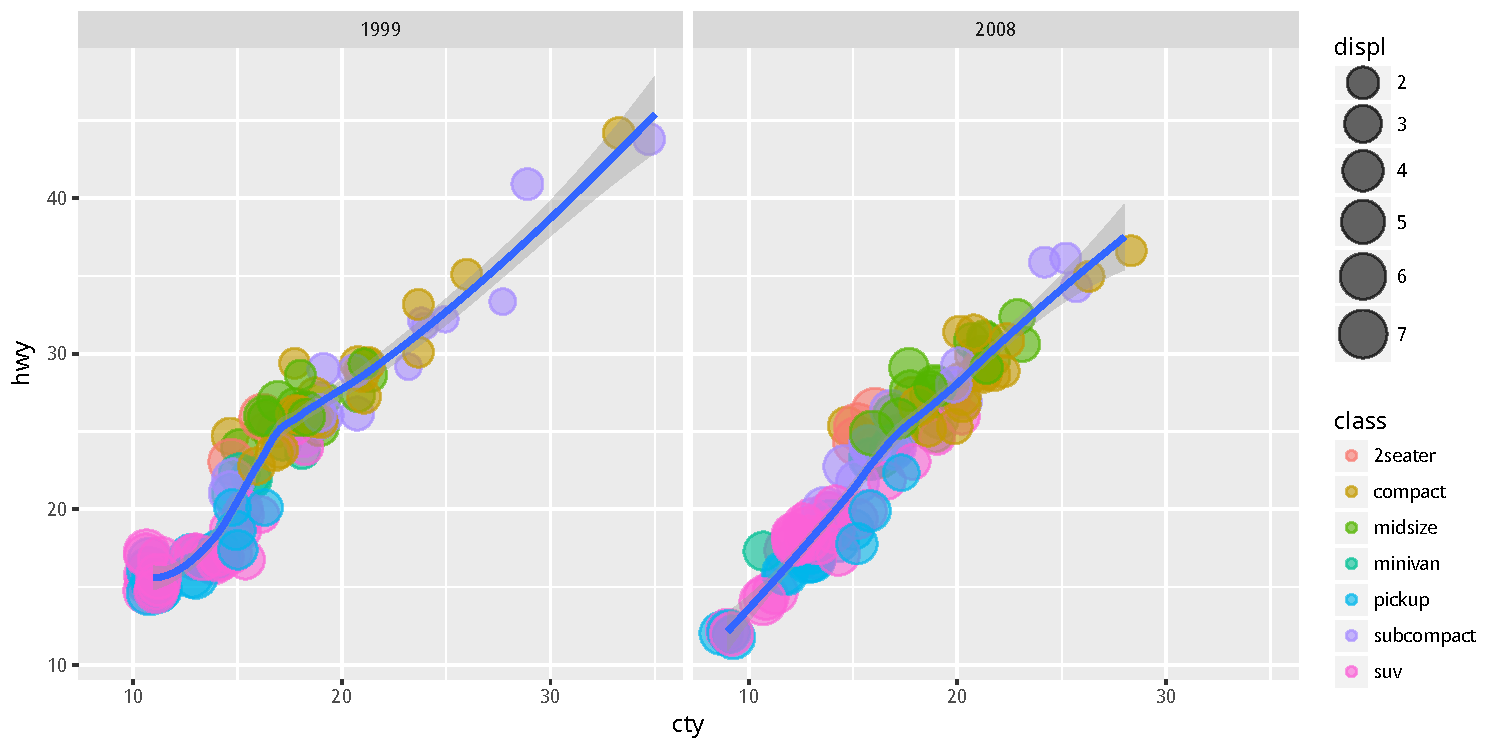
\includegraphics[width=\columnwidth]{ggplot_example4.pdf}
\end{minipage}
\end{onlyenv}

\begin{onlyenv}<5>
\begin{minipage}{\textwidth}
\begin{rcode}
# 第五步:图形微调,调整与图形无关要素,例如添加标题、坐标轴标签、图例标签、注释等
> ggplot(mpg, aes(x=cty, y=hwy))+
     geom_point(aes(colour=class,size=displ),alpha=0.6,position = "jitter")+  
     stat_smooth()+  
     scale_size(range = c(5, 10))+
     facet_wrap(~ year,ncol=2)+
     ggtitle("汽车油耗与型号")+  
     labs(y='每加仑高速公路行驶距离',x='每加仑城市公路行驶距离')+  
     guides(size=guide_legend(title='排量'),colour=guide_legend(title='车型',override.aes=
            list(size=5)))
\end{rcode}
\end{minipage}
\begin{minipage}{\textwidth}
\centering
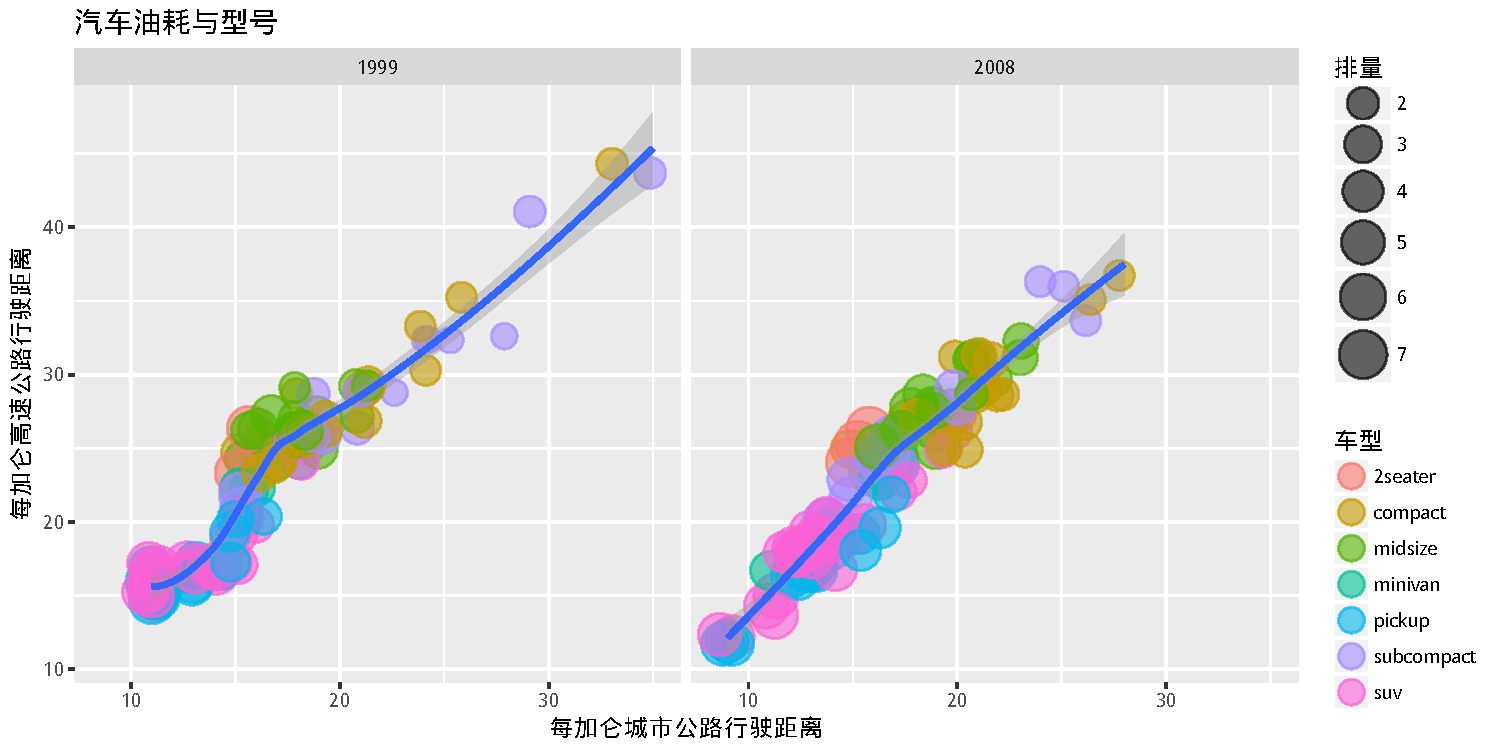
\includegraphics[width=\columnwidth]{ggplot_example5.pdf}
\end{minipage}
\end{onlyenv}

\end{frame}
